\documentclass[11pt]{article}
\usepackage[margin=1in]{geometry}
\usepackage{amsmath,amssymb,amsthm}
\usepackage{graphicx}
\usepackage{float}
\usepackage[onehalfspacing]{setspace}
\usepackage[unicode=true,
 bookmarks=true,bookmarksnumbered=false,bookmarksopen=false,
 breaklinks=false,pdfborder={0 0 0},pdfborderstyle={},backref=false,colorlinks=true]
 {hyperref}
\usepackage{verbatim}
\usepackage{appendix}
\usepackage{mathtools}
\usepackage{url}
\usepackage[authoryear]{natbib}
\usepackage{soul}
\usepackage{tikz}
\usetikzlibrary{calc}
\usepackage{caption}
\usepackage{subcaption}
\usepackage{comment}
\usepackage{ulem}
\usepackage{setspace}
\usepackage[en-US]{datetime2}

\renewcommand{\v}[1]{\ensuremath{\mathbf{#1}}} % for vectors
\newcommand{\gv}[1]{\ensuremath{\mbox{\boldmath$ #1 $}}} 
% for vectors of Greek letters
\newcommand{\uv}[1]{\ensuremath{\mathbf{\hat{#1}}}} % for unit vector
\newcommand{\abs}[1]{\left| #1 \right|} % for absolute value
\newcommand{\avg}[1]{\left< #1 \right>} % for average
\let\underdot=\d % rename builtin command \d{} to \underdot{}
\renewcommand{\d}[2]{\frac{d #1}{d #2}} % for derivatives
\newcommand{\dd}[2]{\frac{d^2 #1}{d #2^2}} % for double derivatives
\newcommand{\pd}[2]{\frac{\partial #1}{\partial #2}} 
% for partial derivatives
\newcommand{\pdd}[2]{\frac{\partial^2 #1}{\partial #2^2}} 
% for double partial derivatives
\newcommand{\pdc}[3]{\left( \frac{\partial #1}{\partial #2}
 \right)_{#3}} % for thermodynamic partial derivatives
\newcommand{\ket}[1]{\left| #1 \right>} % for Dirac bras
\newcommand{\bra}[1]{\left< #1 \right|} % for Dirac kets
\newcommand{\braket}[2]{\left< #1 \vphantom{#2} \right|
 \left. #2 \vphantom{#1} \right>} % for Dirac brackets
\newcommand{\matrixel}[3]{\left< #1 \vphantom{#2#3} \right|
 #2 \left| #3 \vphantom{#1#2} \right>} % for Dirac matrix elements
\newcommand{\grad}[1]{\gv{\nabla} #1} % for gradient
\let\divsymb=\div % rename builtin command \div to \divsymb
\renewcommand{\div}[1]{\gv{\nabla} \cdot \v{#1}} % for divergence
\newcommand{\curl}[1]{\gv{\nabla} \times \v{#1}} % for curl
\newcommand{\stkout}[1]{\ifmmode\text{\sout{\ensuremath{#1}}}\else\sout{#1}\fi}
\newcommand{\msout}[1]{\text{\sout{\ensuremath{#1}}}}
\let\baraccent=\= % rename builtin command \= to \baraccent
\renewcommand{\=}[1]{\stackrel{#1}{=}} % for putting numbers above =
\providecommand{\wave}[1]{\v{\tilde{#1}}}
\providecommand{\fr}{\frac}
\providecommand{\RR}{\mathbb{R}}
\providecommand{\NN}{\mathbb{N}}
\providecommand{\seq}{\subseteq}
\providecommand{\e}{\epsilon}
\newtheorem{prop}{Proposition}
\newtheorem*{lem}{Lemma}
\theoremstyle{definition}
\newtheorem*{dfn}{Definition}
\newenvironment{s}{%\small%
        \begin{trivlist} \item \textbf{Solution}. }{%
            \hspace*{\fill} $\blacksquare$\end{trivlist}}%
\newenvironment{p}{}{}
\DeclareMathOperator*{\argmax}{arg\,max}
\DeclareMathOperator*{\argmin}{arg\,min}

\hypersetup{
	pdftex,
    pdfauthor={Jonathan I. Dingel and friends},     % author
    colorlinks=true,       % false: boxed links; true: colored links
    linkcolor=red,          % color of internal links
    citecolor=black,        % color of links to bibliography
    urlcolor=blue           % color of external links
}

% CUSTOM DEFINITIONS
\urldef{\dingelhomepage}\url{http://faculty.chicagobooth.edu/jonathan.dingel/}
\urldef{\rufemail}\url{jcruf@uchicago.edu}
\newtheorem{proposition}{Proposition}

% IDENTIFYING INFORMATION
\title{Politics and the Provision of Public Goods: Evidence from Chicago}
\author{John C. Ruf \thanks{\rufemail}}
\date{\today}


\begin{document}
\bibliographystyle{../bib/aeanobold}
\maketitle
% -----------------------------------------------
% 	ABSTRACT
% -----------------------------------------------

\begin{abstract}
\begin{spacing}{1.0}
This paper investigates the political economy of conspicuous public spending. 
It defines conspicuous public spending as spending intended to signal competency to voters for electoral gain. 
A simple career-concerns model featuring a tradeoff between conspicuous and inconspicuous expenditures with experience gain demonstrates this effect in a rational-choice framework. 
The model has two critical implications. 
Firstly, unexpected increases in conspicuous expenditures help politicians get re-elected. 
Secondly, less-experienced politicians spend more conspicuously than their established counterparts. 
This paper uses data from Chicago's Aldermanic Menu Program to test these implications. 
The first implication is confirmed via a simple discrete-choice analysis. Differences-in-differences methods further show some evidence for the second implication. 
However, counter to the model, the Differences-in-Differences study shows an effect that decays before the next election.
Furthermore, a regression discontinuity analysis also shows an increase in spending, which is not consistent with the model.
This paper concludes by exploring alternative hypotheses that may be driving the decaying effect.
\end{spacing}
\end{abstract}
\vspace{1cm}
{\small
\noindent \textit{Keywords}: Menu Program, Aldermen, Infrastructure Maintenance \\
\textit{JEL codes}: L98 H72 
}
\thispagestyle{empty}
\newpage
\setcounter{page}{1}

% -----------------------------------------------
% 	BODY
% -----------------------------------------------

%\section{Introduction}

\begin{frame}{Motivation}
    How do local politicians allocate infrastructure maintenance and other key public goods?
    \begin{itemize}
        \item (Glaeser 2019) find a strong shortage of road maintenance in the country: is it a political economy problem?
        \item If local politicians cannot be trusted to maintain key infrastructure and roads, that has important welfare implications for optimal placement of ``large'' welfare enhancing projects.
        \item How prevalent would clientelism be if we allocated public resources in a more decentralized manner?
        \item What are the costs of giving local politicians unilateral control over infrastructure maintenance? What magnitude would the benefits like ``local knowledge'' and ``accountability'' need to be to justify this?
    \end{itemize}
\end{frame}
    
\begin{frame}{What do aldermen do?}
    \begin{center}
    \begin{quotation}
        ``I remember crossing California going west, every street was resurfaced almost every year. They always had brand new lighting and then east of California, where Ald. Bernie Stone would lose the precincts consistently, I mean the streets were in shambles.'' \\
    \end{quotation}
    \end{center}
    \raggedleft{ -Ald. Carlos Ramirez-Rosa (35th Ward).}
    \begin{itemize}
        \item Aldermen as Mini-Mayor over Ward
        \begin{itemize}
            \item City council defers to Ward Alderman all internal issues
            \item Eg. \ snow plows, garbage cleanup, sign permits, business licenses, liquor-moratoriums, and of course, construction and zoning.
            \item A relatively new power that aldermen were granted in 1995 is the ability to allocate \$1.5M in infrastructure ``menu'' requests 
        \end{itemize}
    \end{itemize}
\end{frame}
    
\begin{frame}{What is the Aldermanic Menu Program?}
        Alderman have the power to allocate \$ 1.5M on a variety of infrastructure projects. They are given a map of 311 complaints for guidance.
    \begin{itemize}
        \item  5 primary categories:
        \begin{itemize}
            \item \textbf{Streets/CDOT:} Alley/Road/Sidewalk Resurfacing, speed bump replacement, sign installation, Curb and Gutter fixes, etc. 
            \item \textbf{Crime Prevention and Lighting:} Camera installation and street lights
            \item \textbf{Arts:} Murals and Neighborhood Arts programs
            \item \textbf{Schools:} Direct grants to CPS, Sports Fields, Gardens, Auditoriums, Playgrounds, etc. 
            \item \textbf{Parks, Trees, and Gardens:} Tree planting, public garden formation, and park cleanup programs. 
        \end{itemize}
    \end{itemize}
\end{frame}

\begin{frame}{2017 OIG Audit}
        The office of the inspector general (OIG) conducted an audit of the menu program in 2017.
        The audit was scathing. 
        They recommended dismantling the program and reallocating the funds to a more traditional central planning model.
        The primary findings of the audit are given below.
    \begin{enumerate}
        \item  Menu, which serves as the City's primary residential infrastructure
        program, underfunds residential infrastructure needs and results in
        significant funding disparities relative to need between wards.
        \item   In the years 2012 through 2015, the City permitted aldermen to designate
        \$15.1 million of Menu funds for projects unrelated to core residential
        infrastructure.
        \item CDOT allowed at least \$825,292 in Menu spending on projects falling outside
        the appropriate ward boundaries and did not enforce project selection
        submission deadlines.
    \end{enumerate}
\end{frame}
%\input{./sections/theory.tex}
%\input{./sections/estimation.tex}
%\input{./sections/discussion.tex}
\section{Introduction}\label{sec:Introduction}

Do local politicians use machine-style politics to drive public goods towards their supporters? Is spending bias exacerbated or curbed by local political competition?
Because most municipalities allocate spending through collective decision-making bodies such as councils, it is usually difficult to attribute expenditures to individual politicians.
However, one such program exists in the United States: Chicago's Aldermanic Menu Program.
Through this program, the Chicago Department of Transportation (CDOT) gives each of Chicago's 50 aldermen a \$1.5 million budget, an eponymous ``menu'' of common expenditures, and a map of 311 complaints in their ward.
Using these resources, aldermen allocate funds to infrastructure maintenance, parks, and other public goods within their wards, even if they are not on the ``menu.''

This paper asks whether the menu funding towards each alderman's supporters or detractors changes after the alderman leaves office.
If so, what determines the magnitude of this change? 
To answer this, this paper uses a differences-in-differences design to compare the time trends of each supporting or opposing precinct before and after the alderman leaves office.
There are two cases where parallel trends are likely to hold: in close elections where the incumbent wins by a small margin and in cases where the incumbent is indicted and forced to leave office.
In the former, both wards where the aldermen just barely won and just barely lost should have similar spending trends.
Furthermore, both winning and losing aldermen in these cases should have similar expectations of winning, so they should behave similarly in the run-up to the election.
In the latter, the timing of the in-office indictment is uncertain, so 


This paper makes two contributions, firstly it publicly introduces this setting's data, and secondly it finds cases that supports \cite{dixit_londregan1996}'s theory of machine politics.
\cite{dixit_londregan1996} argue that the key to machine politics is for politicians to be more efficient at allocating public goods to their supporters than their opponents.
If this is the case, then the municipality arrives at a ``machine politics'' equilibrium where the incumbent targets all publics goods to their top supporters.
If there is no particular efficiency towards supporters, the municipality goes to a ``downsian'' equilibrium where both the incumbent and the challenger promise to allocate public goods to the most marginal voters.
This paper offers the first quantitative proof of the rumor that Bernie Stone biasedly allocating his funds.
It shows a large swing in fund allocation to the lowest and highest 20\% of precincts by campaign contributions before and after Stone's 2011 defeat by Debra Silverstein. 
Post-defeat, the bottom 20\% precincts saw a \$20,000 yearly increase in funds, while the top 20\% precincts experienced a decline nearly double of that.
This constitutes a difference of 1.65\% of the budget, or \$21,383 per year.
Finally, the paper finds that the stone case study is not always generalizable to other aldermen.
When examining close elections, the paper finds no significant difference in spending trends between the winning and losing aldermen.
However, when looking at aldermen who retire after being indicted, precincts that supported an indicted alderman saw their budget fraction decrease by 1.14pp after his/her removal from office, while those that did not saw a 2.59pp increase, amounting to a total difference of \$56,000 difference each year between the two groups.


Section~\ref{sec:background} describes the program's history, its rules, and its 2017 audit.
Section~\ref{sec:lit_review} describes the public economics literature on public goods allocation and lobbying and the spatial and urban economics literature on infrastructure allocation and how this paper relates to both literatures.
Section~\ref{sec:data_description} describes how the menu program data was collected, its summary statistics, and depicts an aggregate map of menu spending across Chicago for the past decade.
Section~\ref{sec:case_study} presents descriptive data for the case study of Alderman Bernie Stone, rumored to favor supporters with menu program funds. 
Section~\ref{sec:empframe} explains this paper's empirical strategy to determine if the Stone case study can be generalized to other aldermen.
Section~\ref{sec:results} shows the results of said empirical strategy, which finds that aldermen removed or retired due to criminal indictments, which has similar results to the Stone case study. 
However, this does not generalize to competitive elections.
The results from the indictment-based differences-in-differences design are statistically weak and sensitive to the number of precincts included, but are economically large and significant.
Section~\ref{sec:conclusions} concludes.


\section*{Data}
The first data-set employed is web-scraped Aldermanic voting data. This data set contains 123 observations of determining election outcomes. 
Determining election indicates that an election determined who got the office. 
We remove elections where the general election outcome became a runoff to avoid double-counting. 
For the discrete-choice modeling, we use a reduced form of the Aldermanic voting data, with only observations from 2015 and 2019, so we have data on off-menu expenditures from the year before the election. 
Secondly, there are Aldermanic menu expenditures, which contain the yearly allotted allocations from Aldermen and their respective locations from 2012 to 2020. 
This data set contains 450 ward-year observations of the amount of money spent on off-menu items and on-menu items. 
For the DiD analysis, we will use the entire 450 observation data set, but for the regression discontinuity study, we will use only the 123 observations that correspond to the year after an election. 
This data-set comes from the Office of Budget and Management of the city of Chicago \cite{MenuProgramChoices}. 

The data set employed for the regression discontinuity analysis consists of 123 electoral observations across three elections. 
We can see a large standard deviation of off-menu expenditures consisting of approximately 10\% of the budget each alder-person is allocated. 
Furthermore, we can see that, on average, we expect the electoral outcomes of these contests to be heavily skewed towards the incumbent, with an average incumbent vote share of 65.5\%. The summary statistics for the regression discontinuity is below:


% Table created by stargazer v.5.2.3 by Marek Hlavac, Social Policy Institute. E-mail: marek.hlavac at gmail.com
% Date and time: Tue, Jan 24, 2023 - 08:34:01 PM
\begin{table}[!htbp] \centering 
  \caption{} 
  \label{} 
\begin{tabular}{@{\extracolsep{5pt}}lccccc} 
\\[-1.8ex]\hline 
\hline \\[-1.8ex] 
Statistic & \multicolumn{1}{c}{N} & \multicolumn{1}{c}{Mean} & \multicolumn{1}{c}{St. Dev.} & \multicolumn{1}{c}{Min} & \multicolumn{1}{c}{Max} \\ 
\hline \\[-1.8ex] 
off\_menu & 105 & 49,364.090 & 118,693.100 & 0.000 & 705,155.000 \\ 
votepct & 105 & 59.639 & 11.130 & 32.262 & 86.038 \\ 
\hline \\[-1.8ex] 
\end{tabular} 
\end{table} 


The histogram of off-menu expenditures data employed in the regression discontinuity is below. 
In this, we see that the vast majority of wards spend \$0 on off-menu items, but a small minority of alderpersons seem to use off-menu expenditures. 
We also see that the right tail of the distribution is quite long, so not only are off-menu expenditures rare, but the ward may be spending a large amount of money when they happen.

\begin{figure}[H]
    \centering
    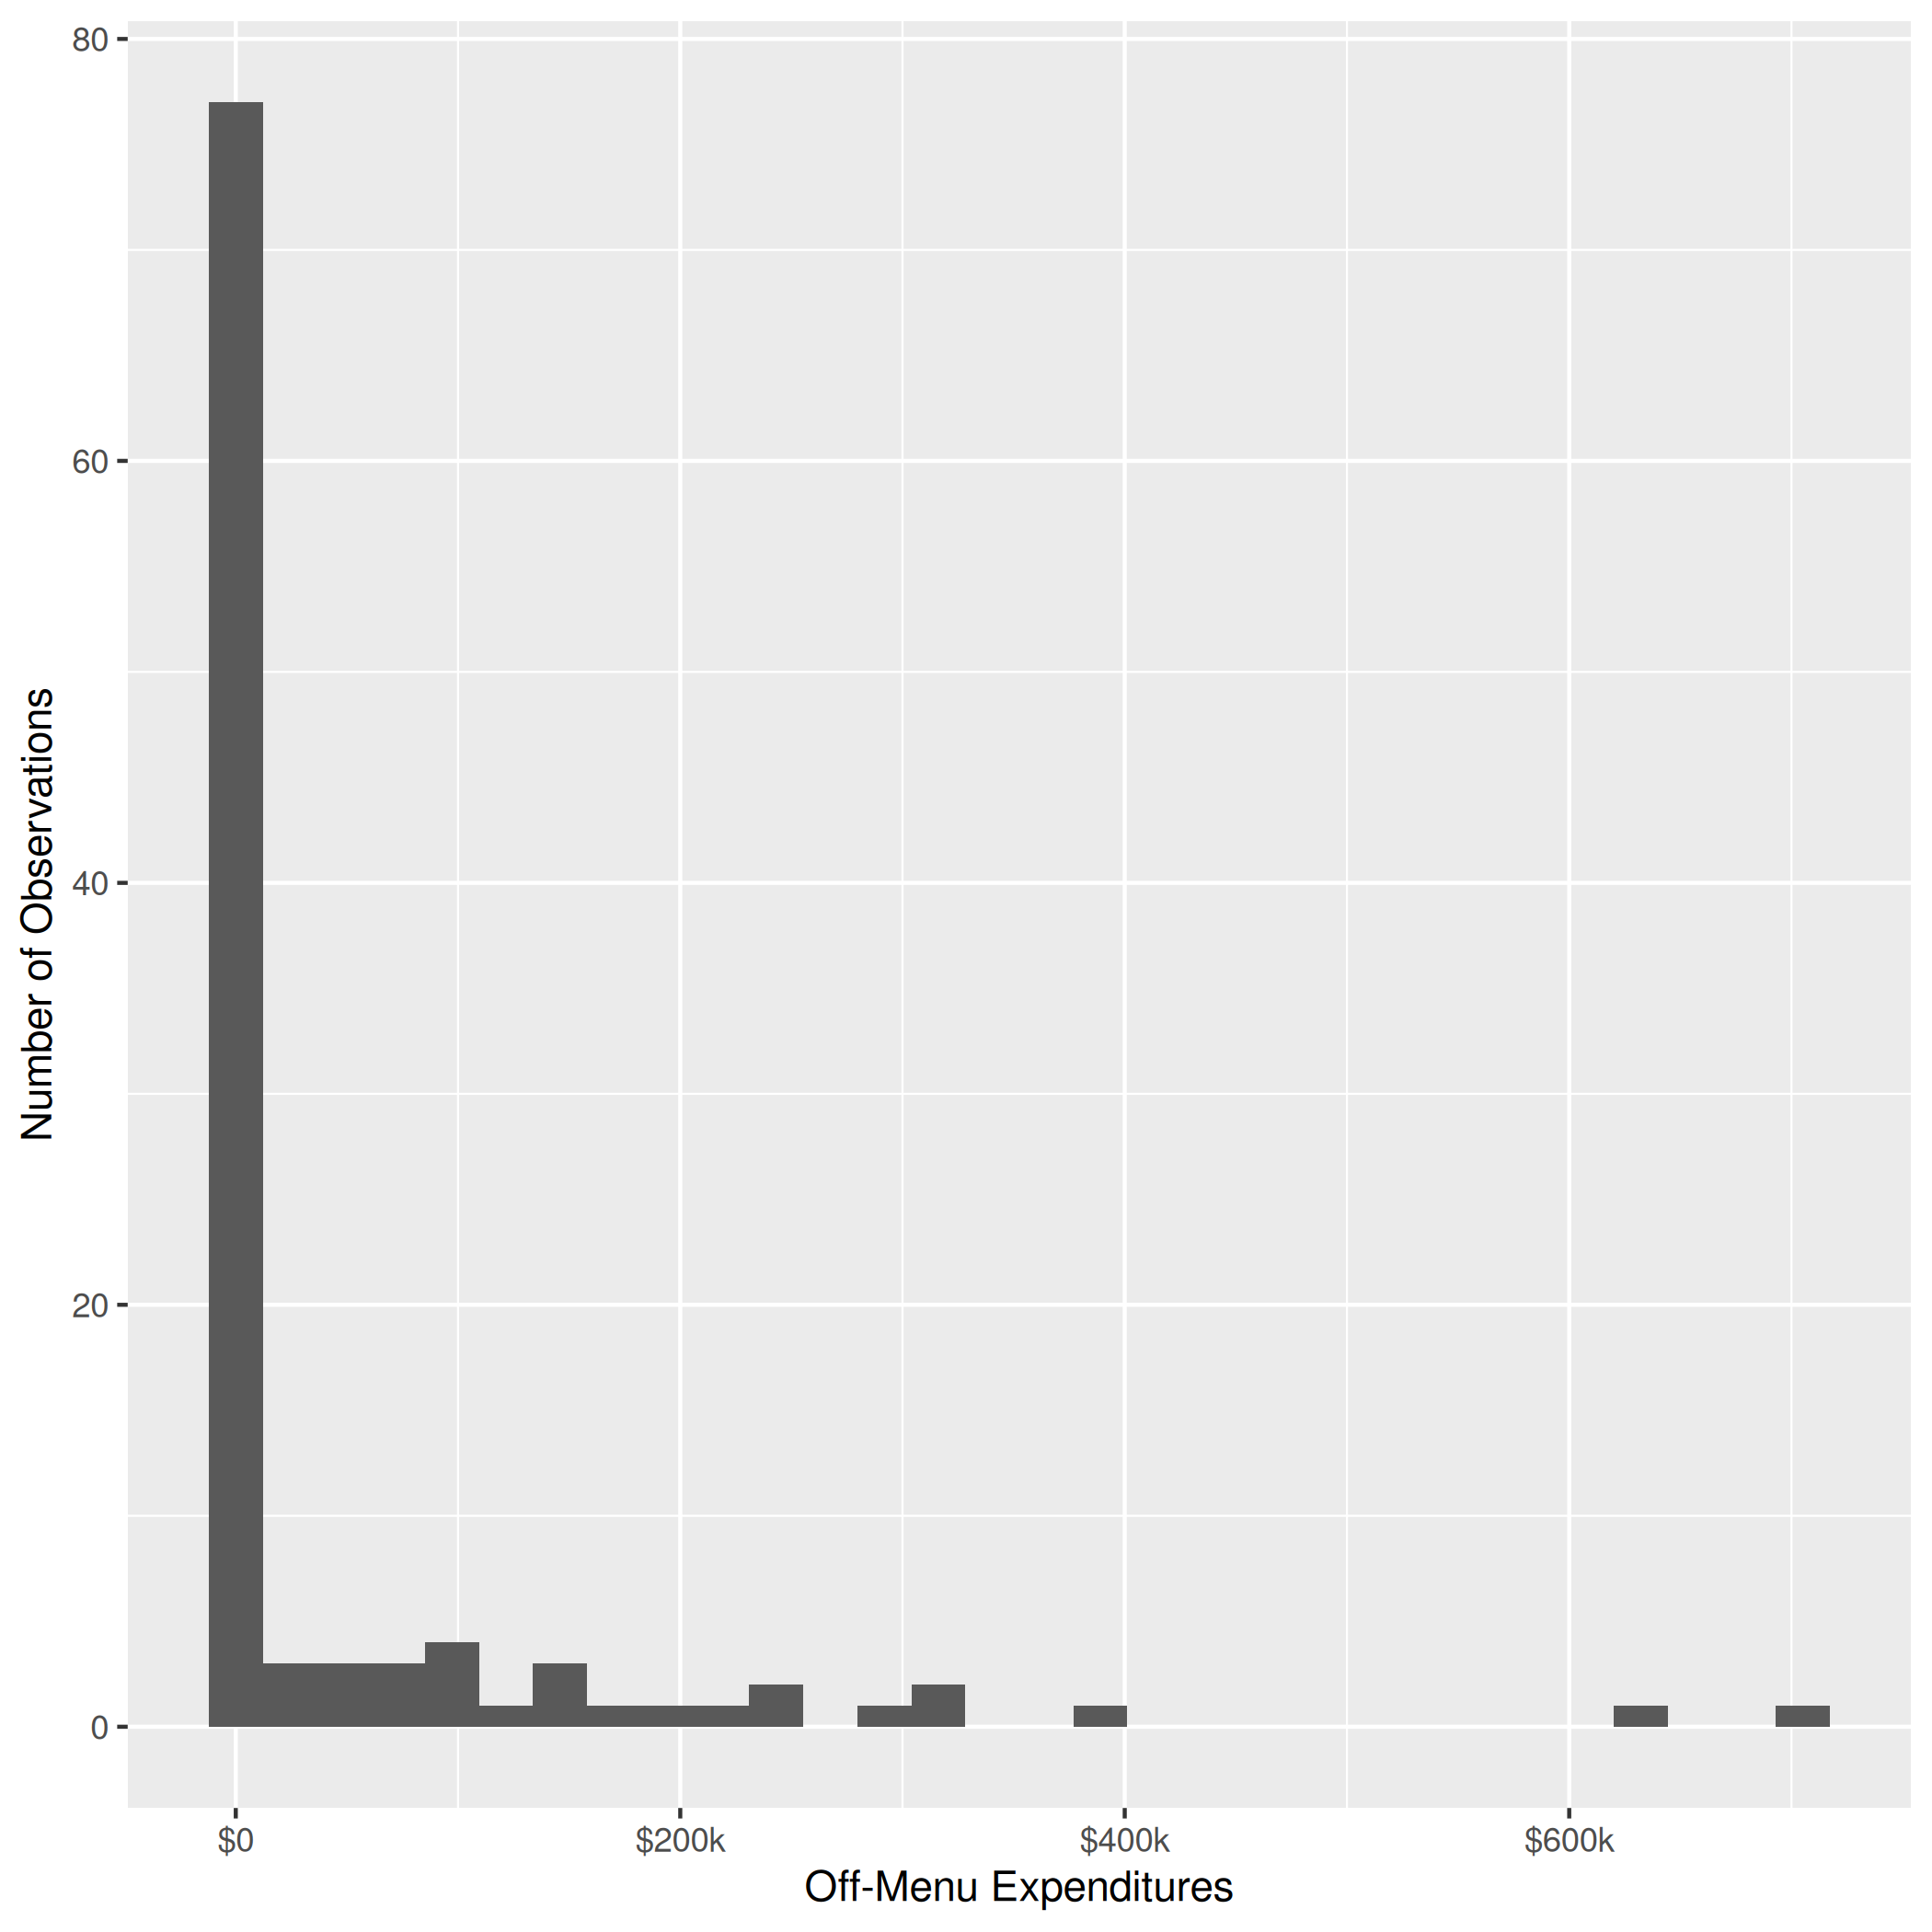
\includegraphics[scale=1]{input/off_menu_expenditures_histogram.png}
    \caption{Histogram of Off-Menu expenditures in 2012, 2016, and 2020 for the RD Analysis}
    \label{fig:my_label}
\end{figure}

A histogram of incumbent vote-shares used in the regression discontinuity analysis is shown below. 
Here we see that the distribution is quite irregular, featuring what seems to be a large discontinuity at the cutoff of 50\% with large density discontinuities elsewhere. 
The histogram shows that the data does not easily fit into a, say, a normal or some other kind of distribution. 
This is likely a reflection of the low number of observations.  

\begin{figure}[H]
    \centering
    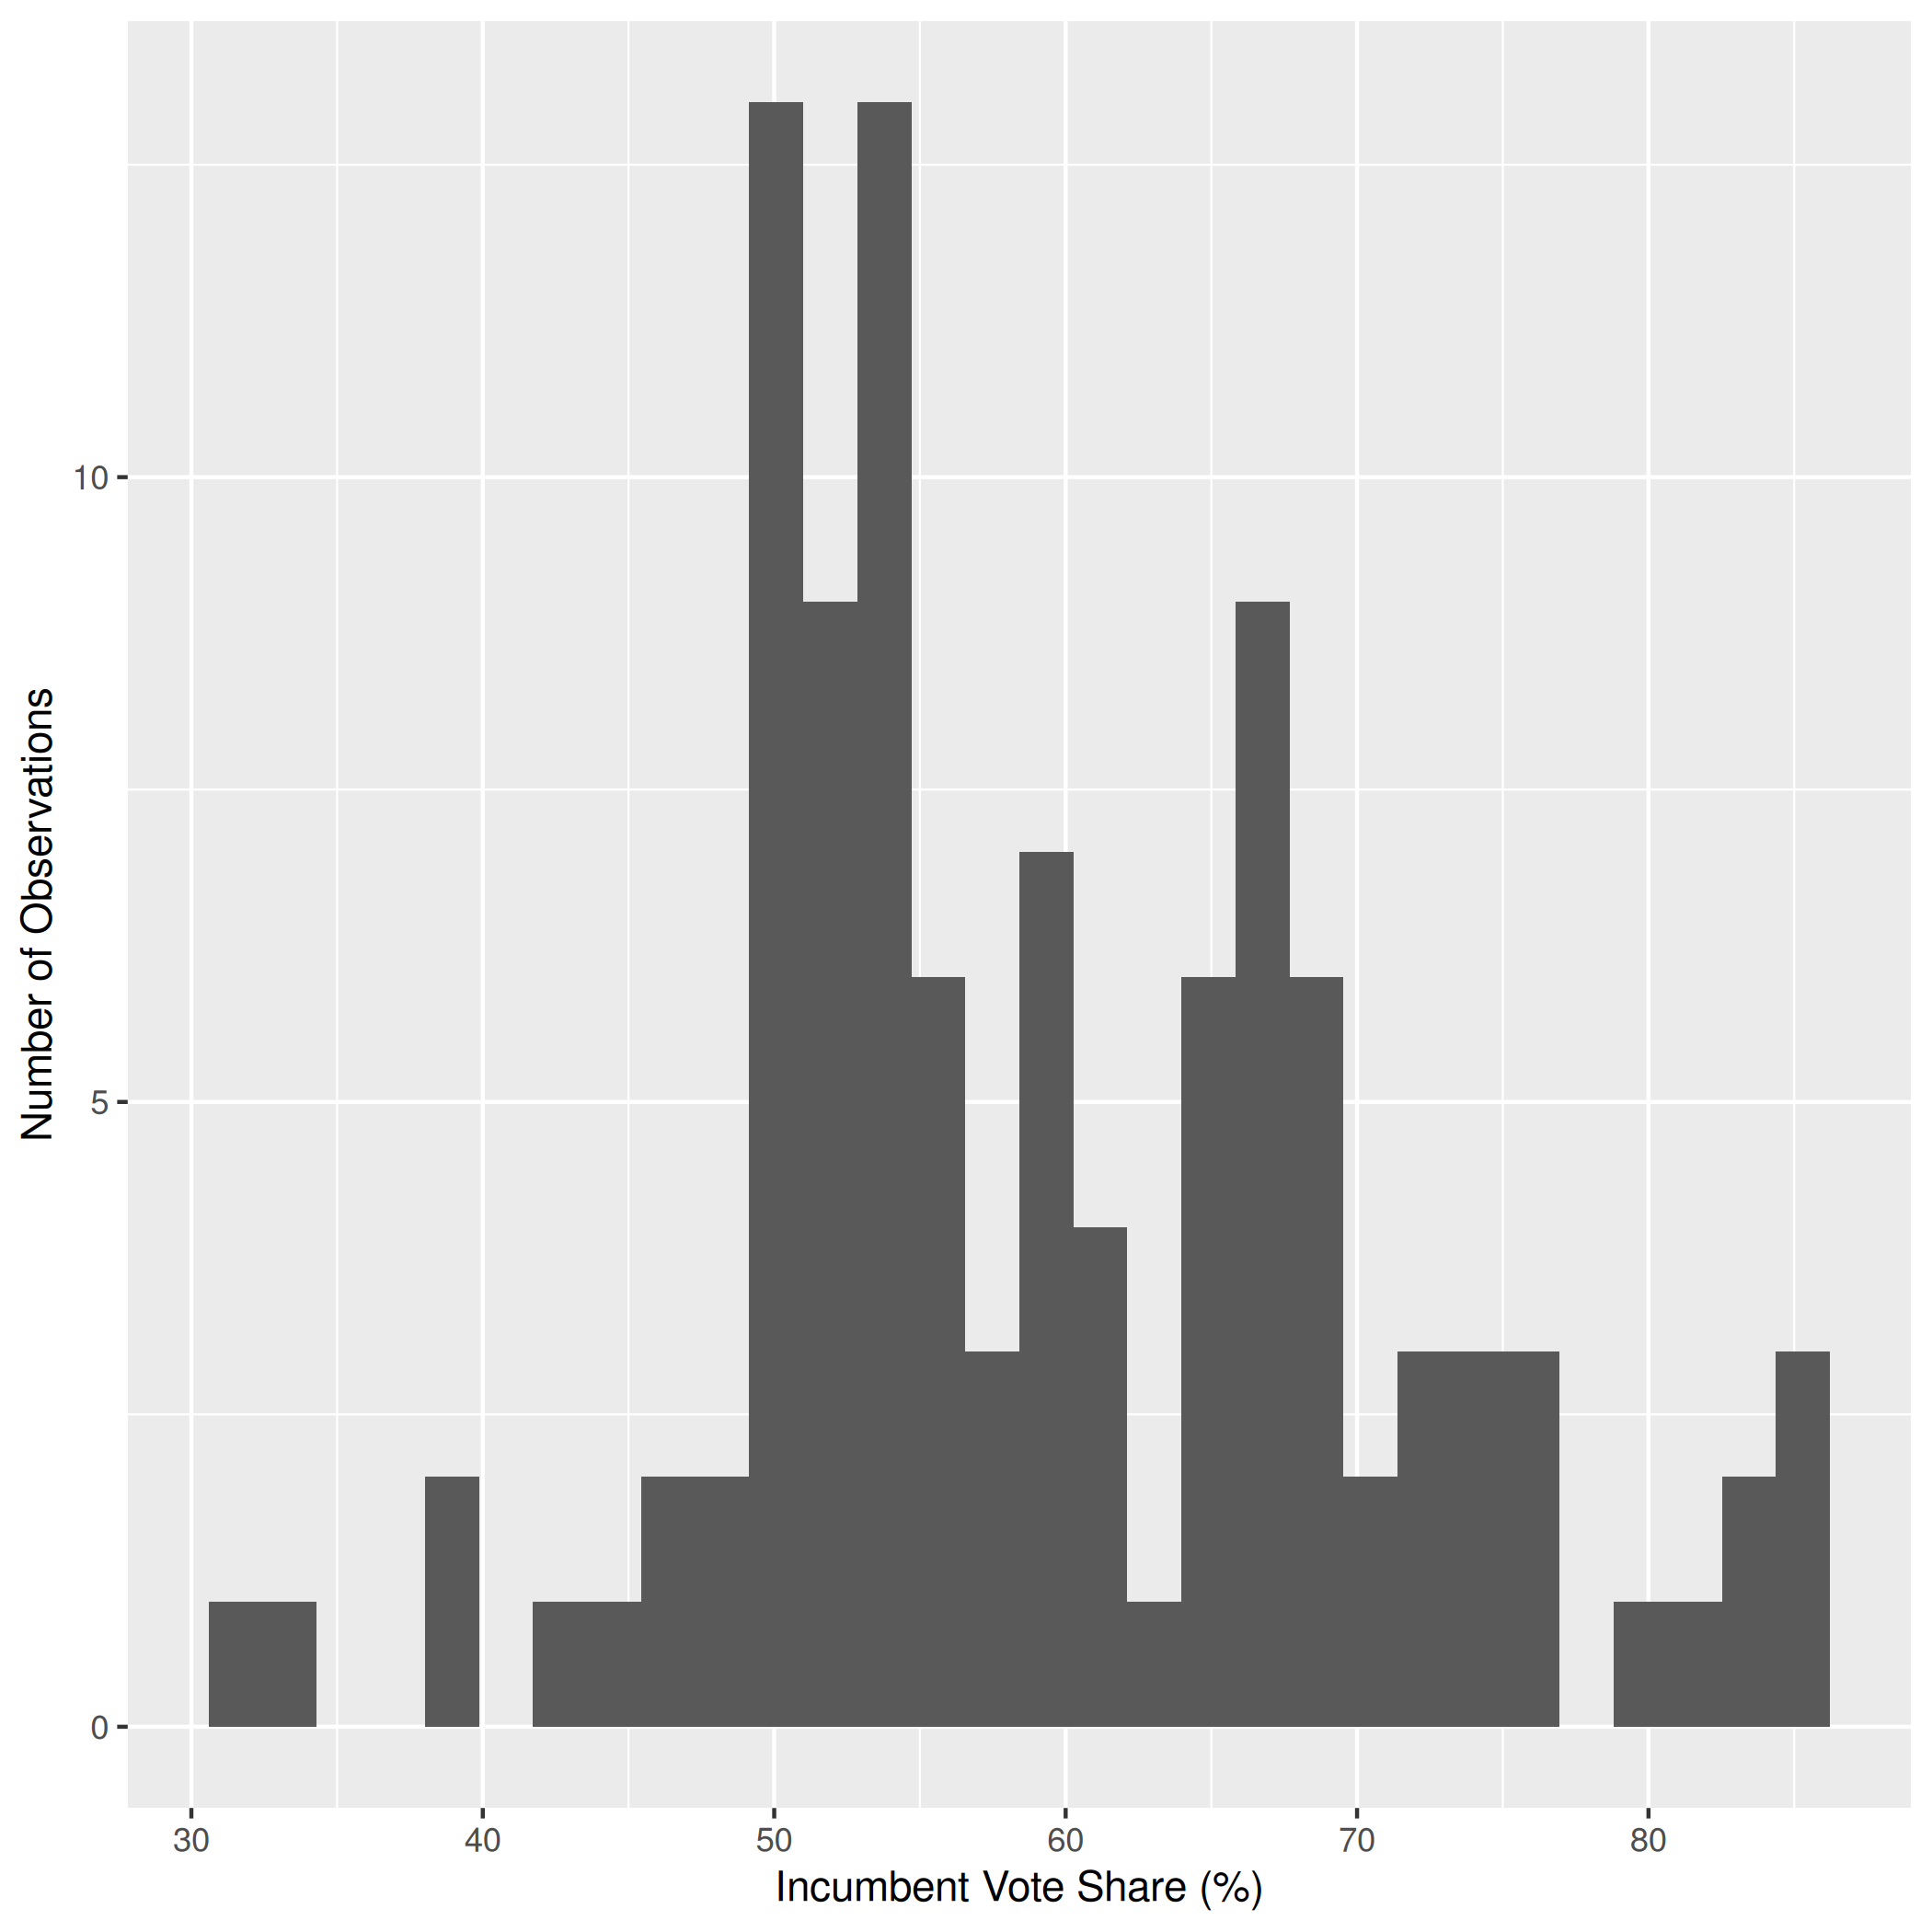
\includegraphics[scale=1]{input/voteshare_histogram.png}
    \caption{Histogram of Incumbent Voteshares in 2011, 2015, and 2019 for the RD analysis}
    \label{fig:my_label}
\end{figure}

The Differences-in-differences data set comprises 450 observations of off-menu expenditures across 50 wards over nine years from 2012-2020. 
Twelve wards are ``treated'' with a leaving incumbent, of which six lost the election, and six retired \cite{election_results}. 
From the summary statistics of the data below, we can see that the treatment group makes up approximately a quarter of the data set and that average off-menu expenditures are lower in the group of wards that had an alderman retire or defeated in a reelection attempt. 

\begin{table}[H] \centering 
  \caption{Summary Statistics for Diff-in-Diff Analysis} 
  \label{} 
\begin{tabular}{@{\extracolsep{5pt}} cccccc} 
\\[-1.8ex]\hline 
\hline \\[-1.8ex] 
 Treatment Group & N & Mean & St. Dev & Min & Max \\ 
\hline \\[-1.8ex] 
treated & 108 & 38554.80 & 94170.02 & 0 & 550000 \\ 
untreated & 342 & 66857.15 & 129705.34 & 0 & 705155 \\ 
\hline \\[-1.8ex] 
\end{tabular} 
\end{table} 


A histogram is presented below for the off-menu expenditures featured in the figure below. 
From this, we can see that the data is similar to the regression discontinuity data set. 
There is a long right tail; most observations are clustered around or directly at zero. 

\begin{figure}[H]
    \centering
    \includegraphics[scale=1]{input/did_hist.png}
    \caption{Off-Menu Expenditures per Unit Year for the Diff-in-Diff Analysis}
    \label{fig:my_label}
\end{figure}


\section*{Bernie Stone Case Study}
This section discusses the Bernie Stone case study, which is the primary motivation for this paper.
Bernie Stone was an alderman in Chicago's 50th ward from 1973 to 2011.
He was well known for his, ``political philosophy.''

\begin{quotation}
    ``You take care of the people who take care of you — you know, the people who voted for you, That’s not Chicago politics, that’s Politics 101.'' - Alderman Bernie Stone (50th ward), Quoted from~\cite{BGA_berniequote}
\end{quotation}

In fact an alderman who grew up in the 50th ward once remarked that,

\begin{quotation}
    ``Well, I grew up in the 50th Ward and you know, God bless [the late former Ald.] Bernie Stone, may he rest in peace, but I remember crossing California going west, every street was resurfaced almost every year. They always had brand new lighting and then east of California, where he would lose the precincts consistently, I mean the streets were in shambles. Many people felt he was spending the bulk of the menu money west of California, where he was getting the bulk of the vote.'' - Alderman Carlos Ramirez-Rosa (35th Ward), Quoted from~\cite{ramirezrosaquote}
\end{quotation}

This quote is a clear example of the type of behavior that this paper seeks to investigate.
This phenomena could not be verified previously because the data was not made publicly available. 
Furthermore, the data that did exist, was in the form of PDFs, which are not easily machine readable.
Thus this paper is the first to put numbers to this anectdotal evidence.
First we can look at a map of the precincts that supported Stone financially and electorally.
Below in Figure~\ref{fig:stone_support_maps} we can see the precincts that supported Stone in the 2007 runoff election and the precincts that gave Stone the most individual contributions.
In both maps we can clearly see that the south western portion of the ward is the most supportive of Stone, on average.
\begin{figure}[H]
    \centering
    % First subfigure
    \begin{subfigure}[b]{0.45\textwidth} % [b] aligns at the bottom
    \includegraphics[width=\textwidth]{input/contribution_map_stone_ward_50_2003_2011.png}
    \caption{Campaign contributions to Alderman Stone, 2003-2011}
    \end{subfigure}
    \hfill % This adds some space between the two subfigures
    % Second subfigure
    \begin{subfigure}[b]{0.45\textwidth}
    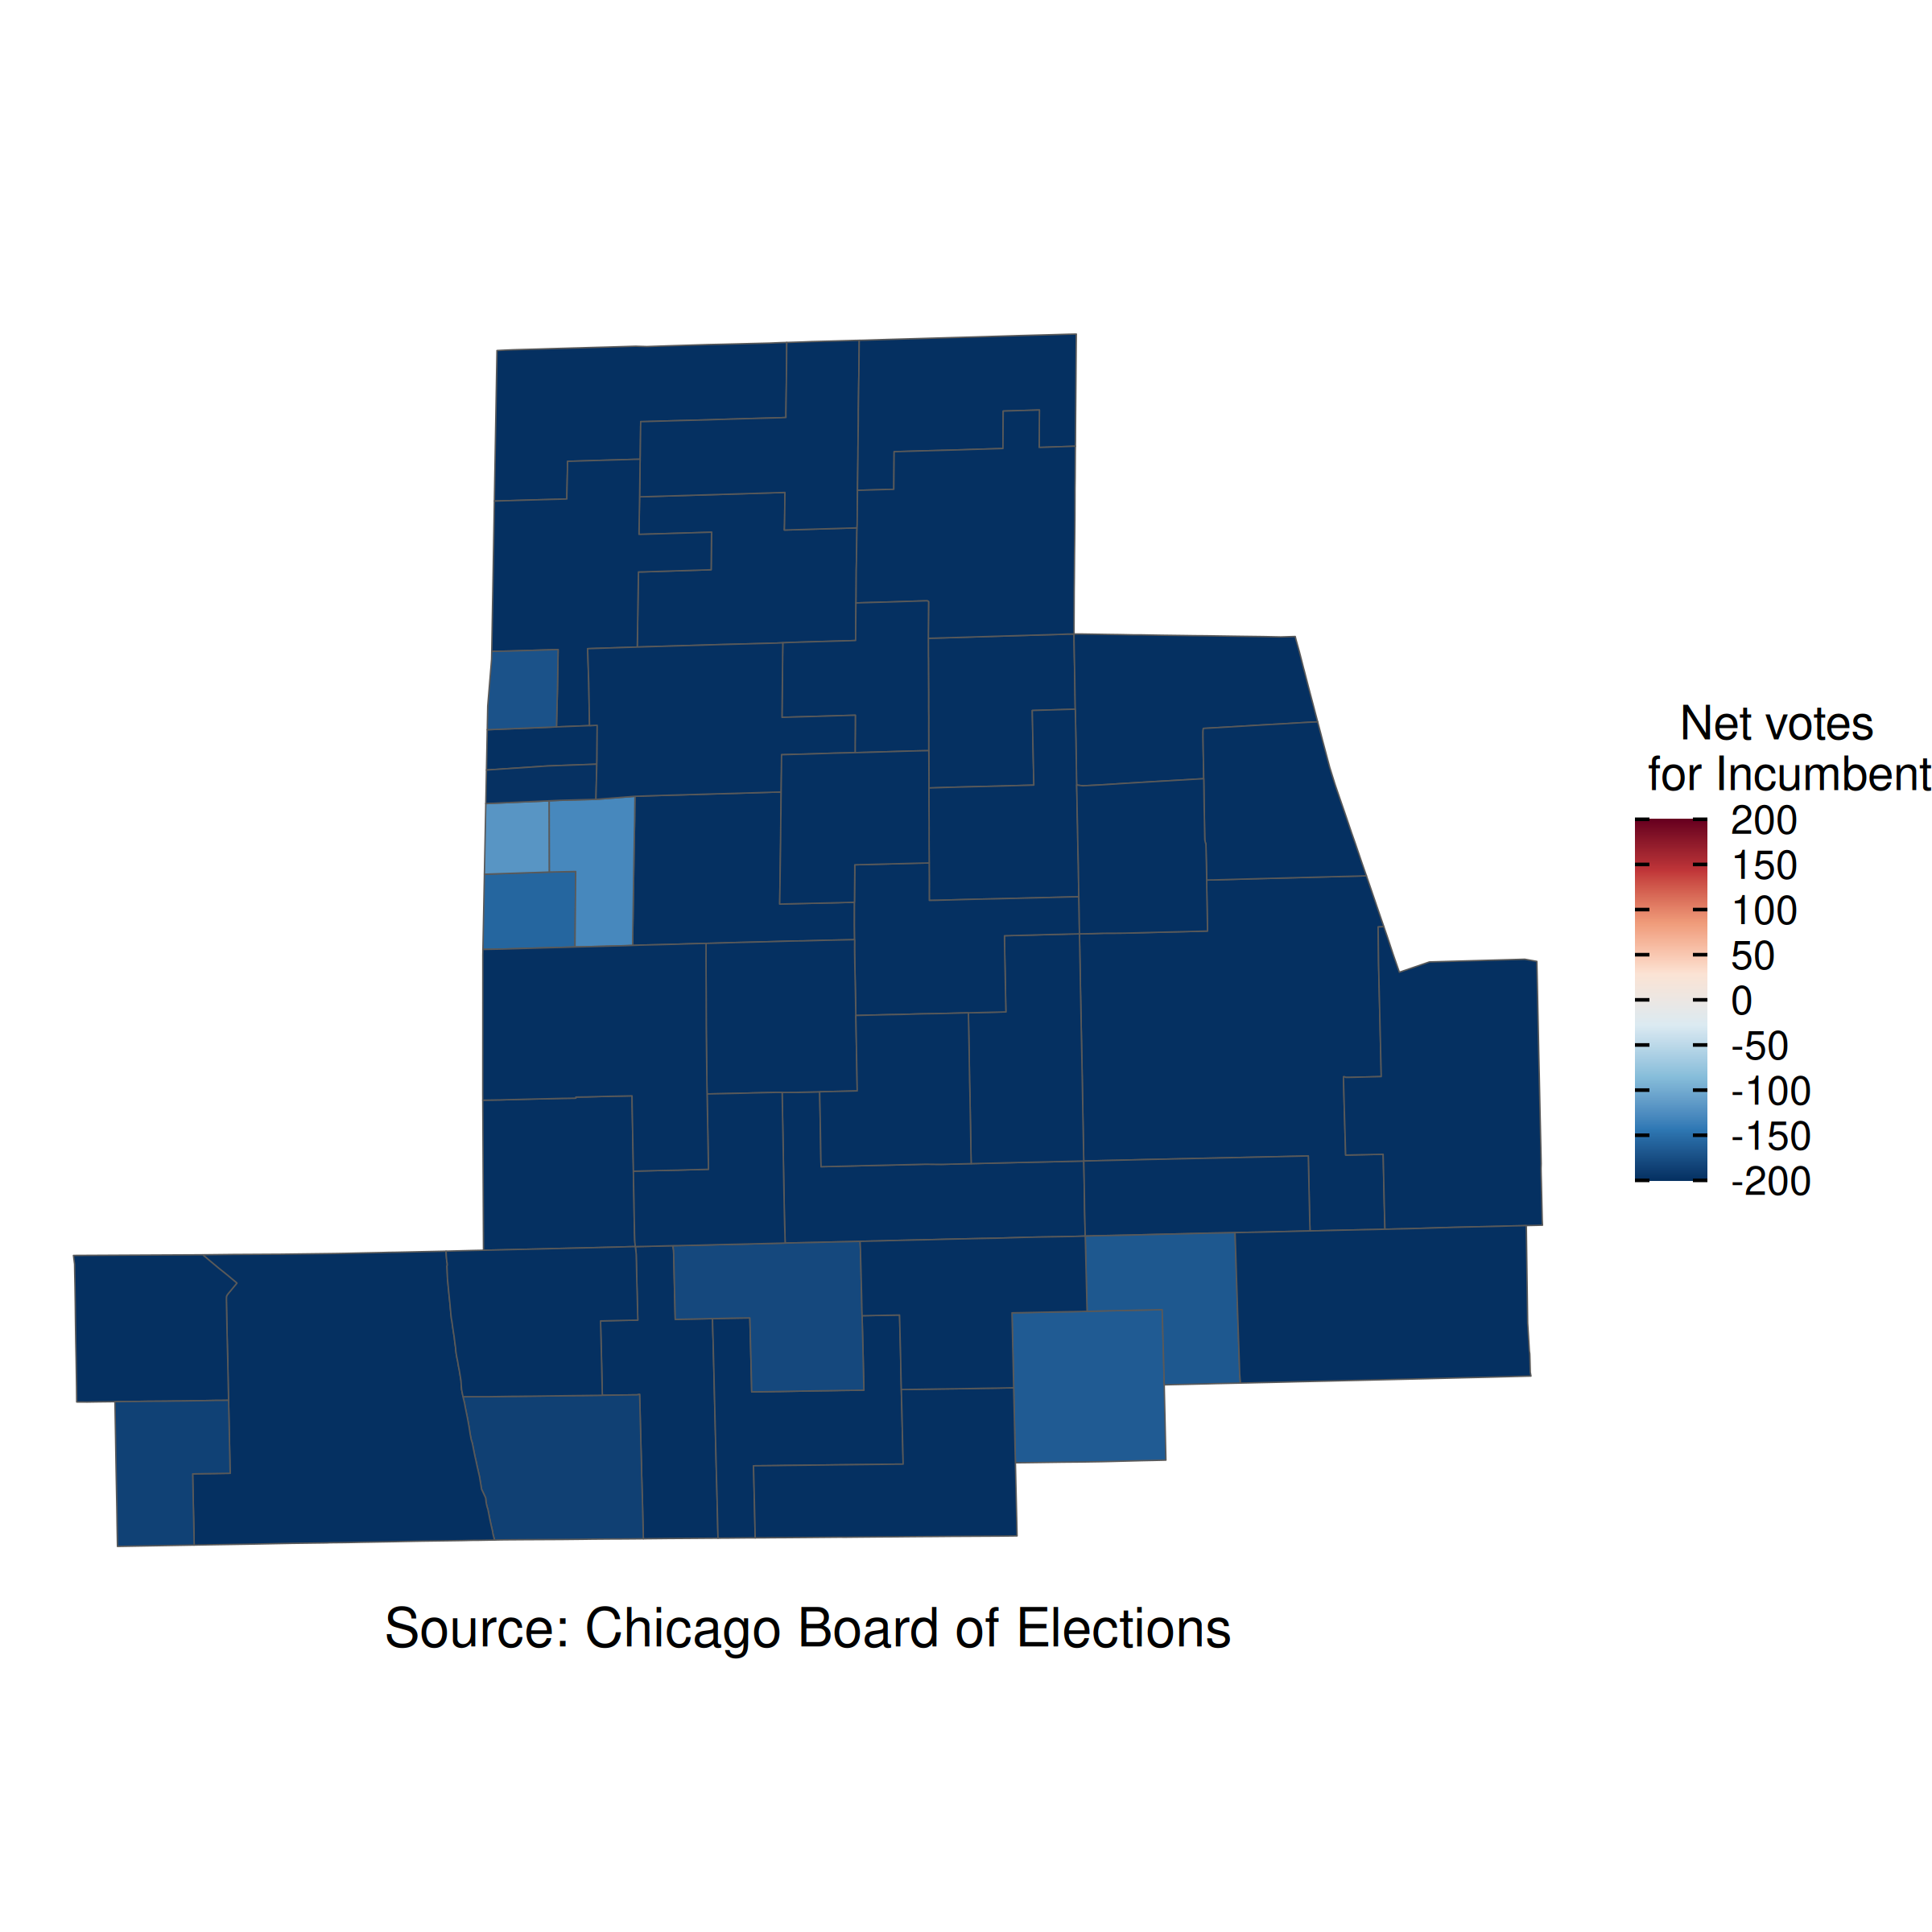
\includegraphics[width=\textwidth]{input/ward_50_2007_runoff_incumbent_precinct_results.png}
    \caption{Net votes for Alderman Stone, 2007}
    \end{subfigure}
    \caption{Distribution of Spending per Precinct for both ward maps in the dataset}
    \label{fig:stone_support_maps}
\end{figure}

Next, we can look at a time series of the spending per precinct for the 50th ward. 
There are approximately 44 precincts in the 50th ward, so Figure~\ref{fig:stone_spending_timeline} gathers the top and bottom quintile of precincts by contributions to Stone and shows average fraction of the total located budget spent in each quintile. 
``other'' refers to all the precincts that are not in the top or bottom quintile.

\begin{figure}[H]
    \centering
    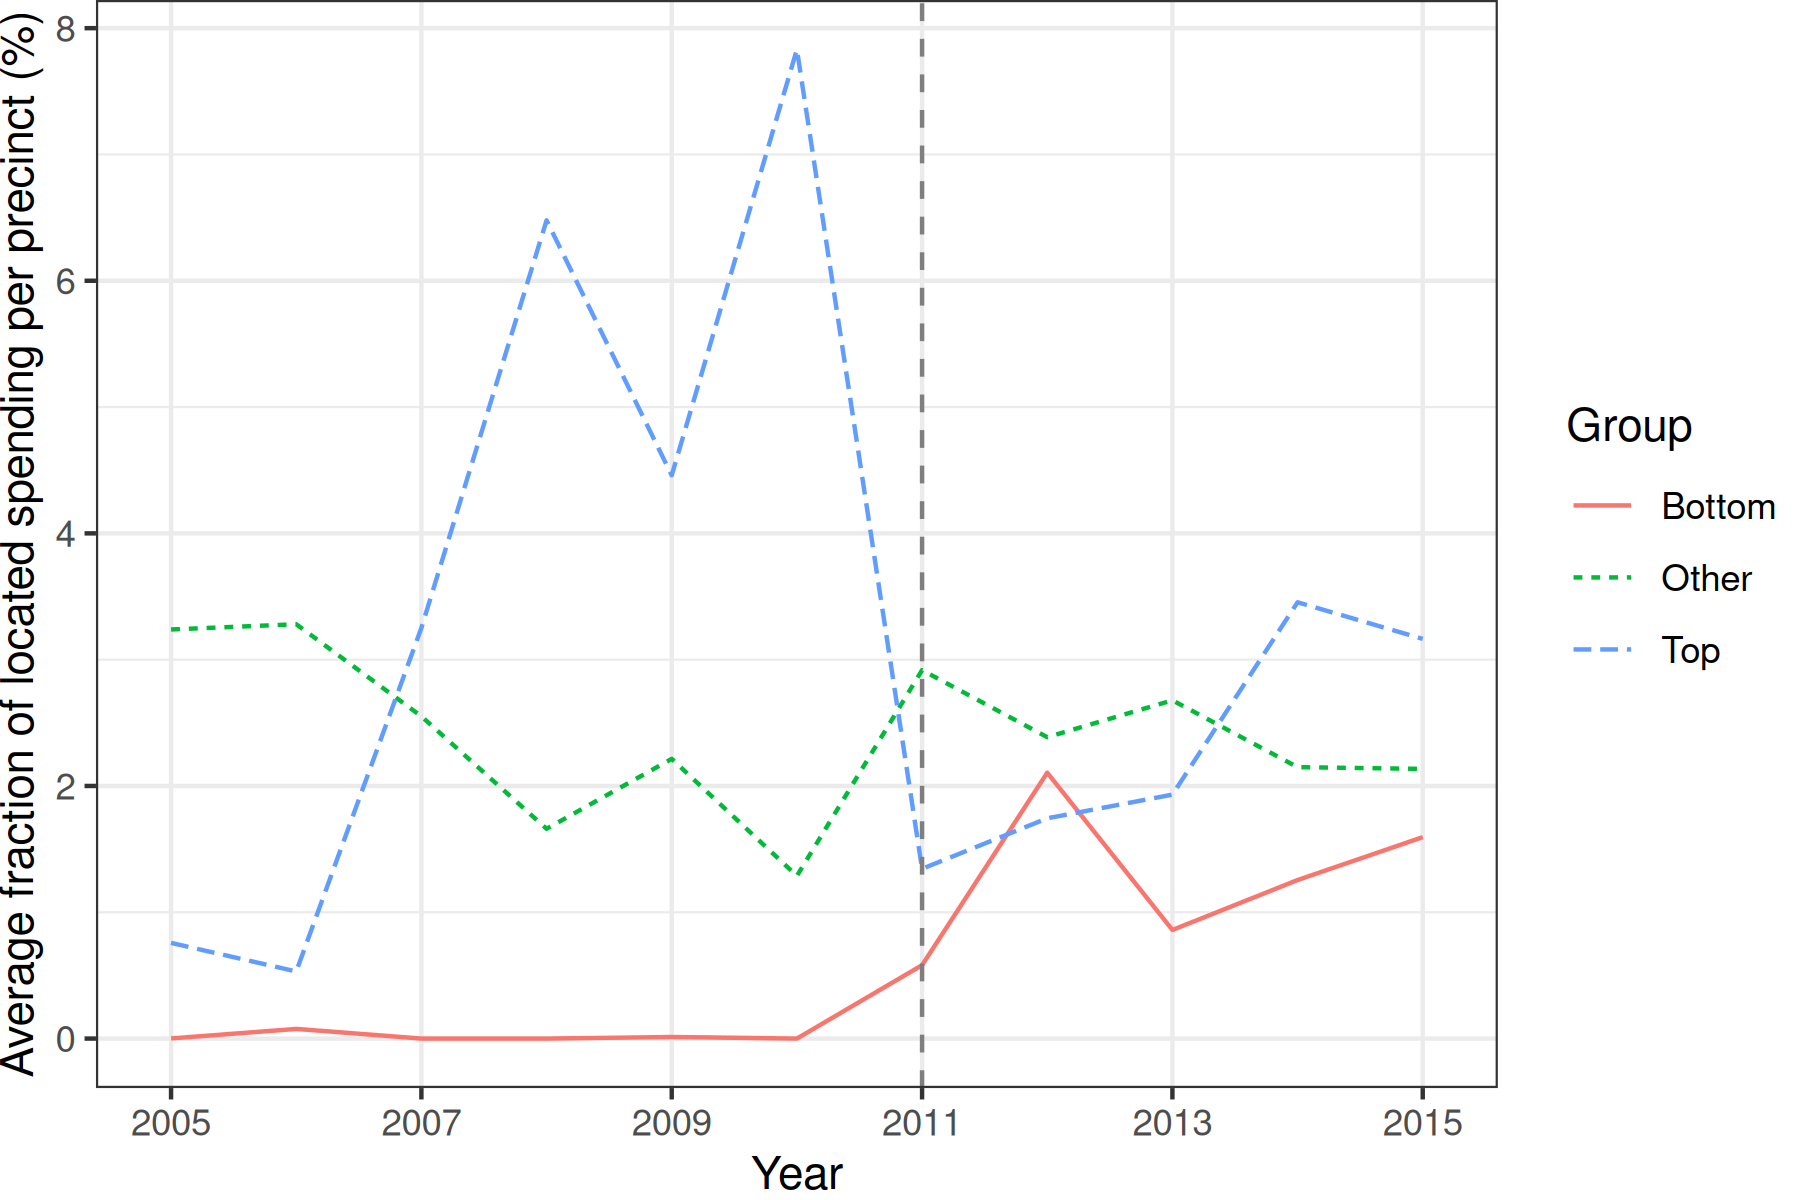
\includegraphics[width=0.8\textwidth]{input/ward_50_contribution_8_precincts_timeline.png}
    \caption{Average Spending per Precinct in the 50th Ward, 2005-2016}
    \label{fig:stone_spending_timeline}
\end{figure}

Finally, we can look at the 50th ward's spending per precinct in the years leading up to and following Stone's defeat in 2011.
This shows a clear shift in spending from the south-western portion of the ward, to a roughly even distribution across the ward.

\begin{figure}[H]
    \centering
    % First subfigure
    \begin{subfigure}[b]{0.45\textwidth} % [b] aligns at the bottom
    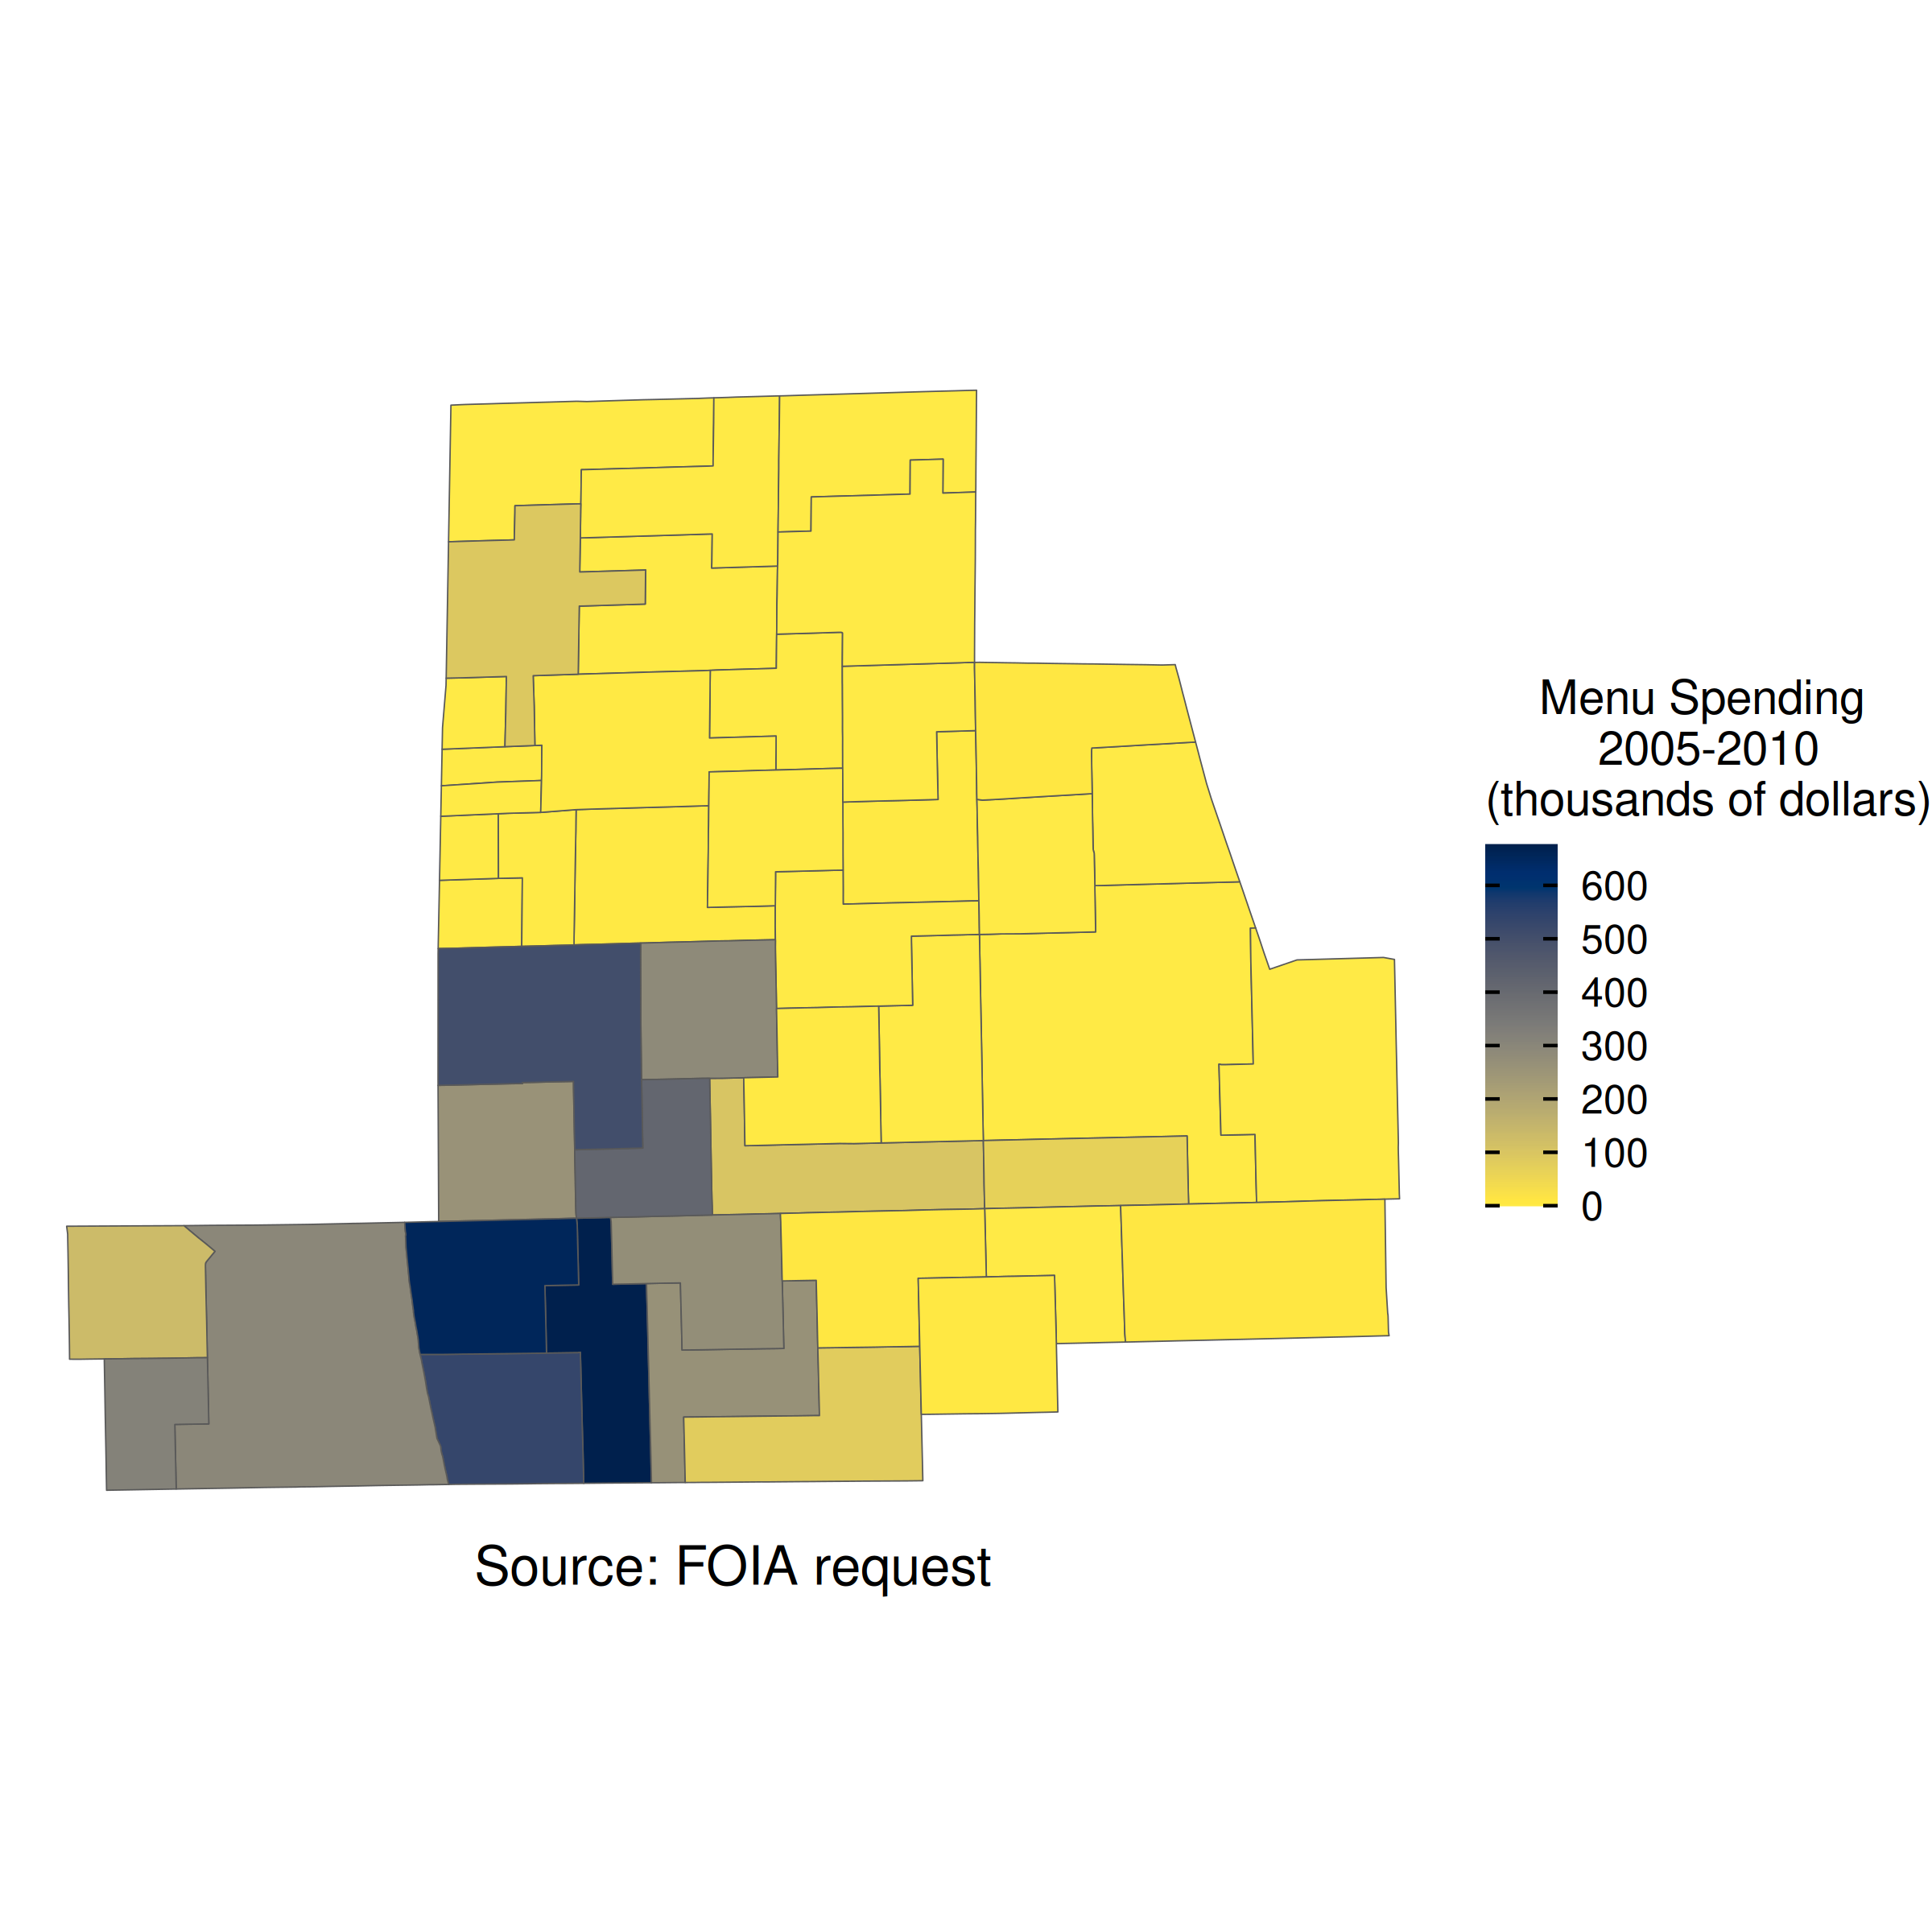
\includegraphics[width=\textwidth]{input/ward_50_menu_map_2005_2010.png}
    \caption{50th Ward Menu Allocation, 2005-2010}
    \end{subfigure}
    \hfill % This adds some space between the two subfigures
    % Second subfigure
    \begin{subfigure}[b]{0.45\textwidth}
    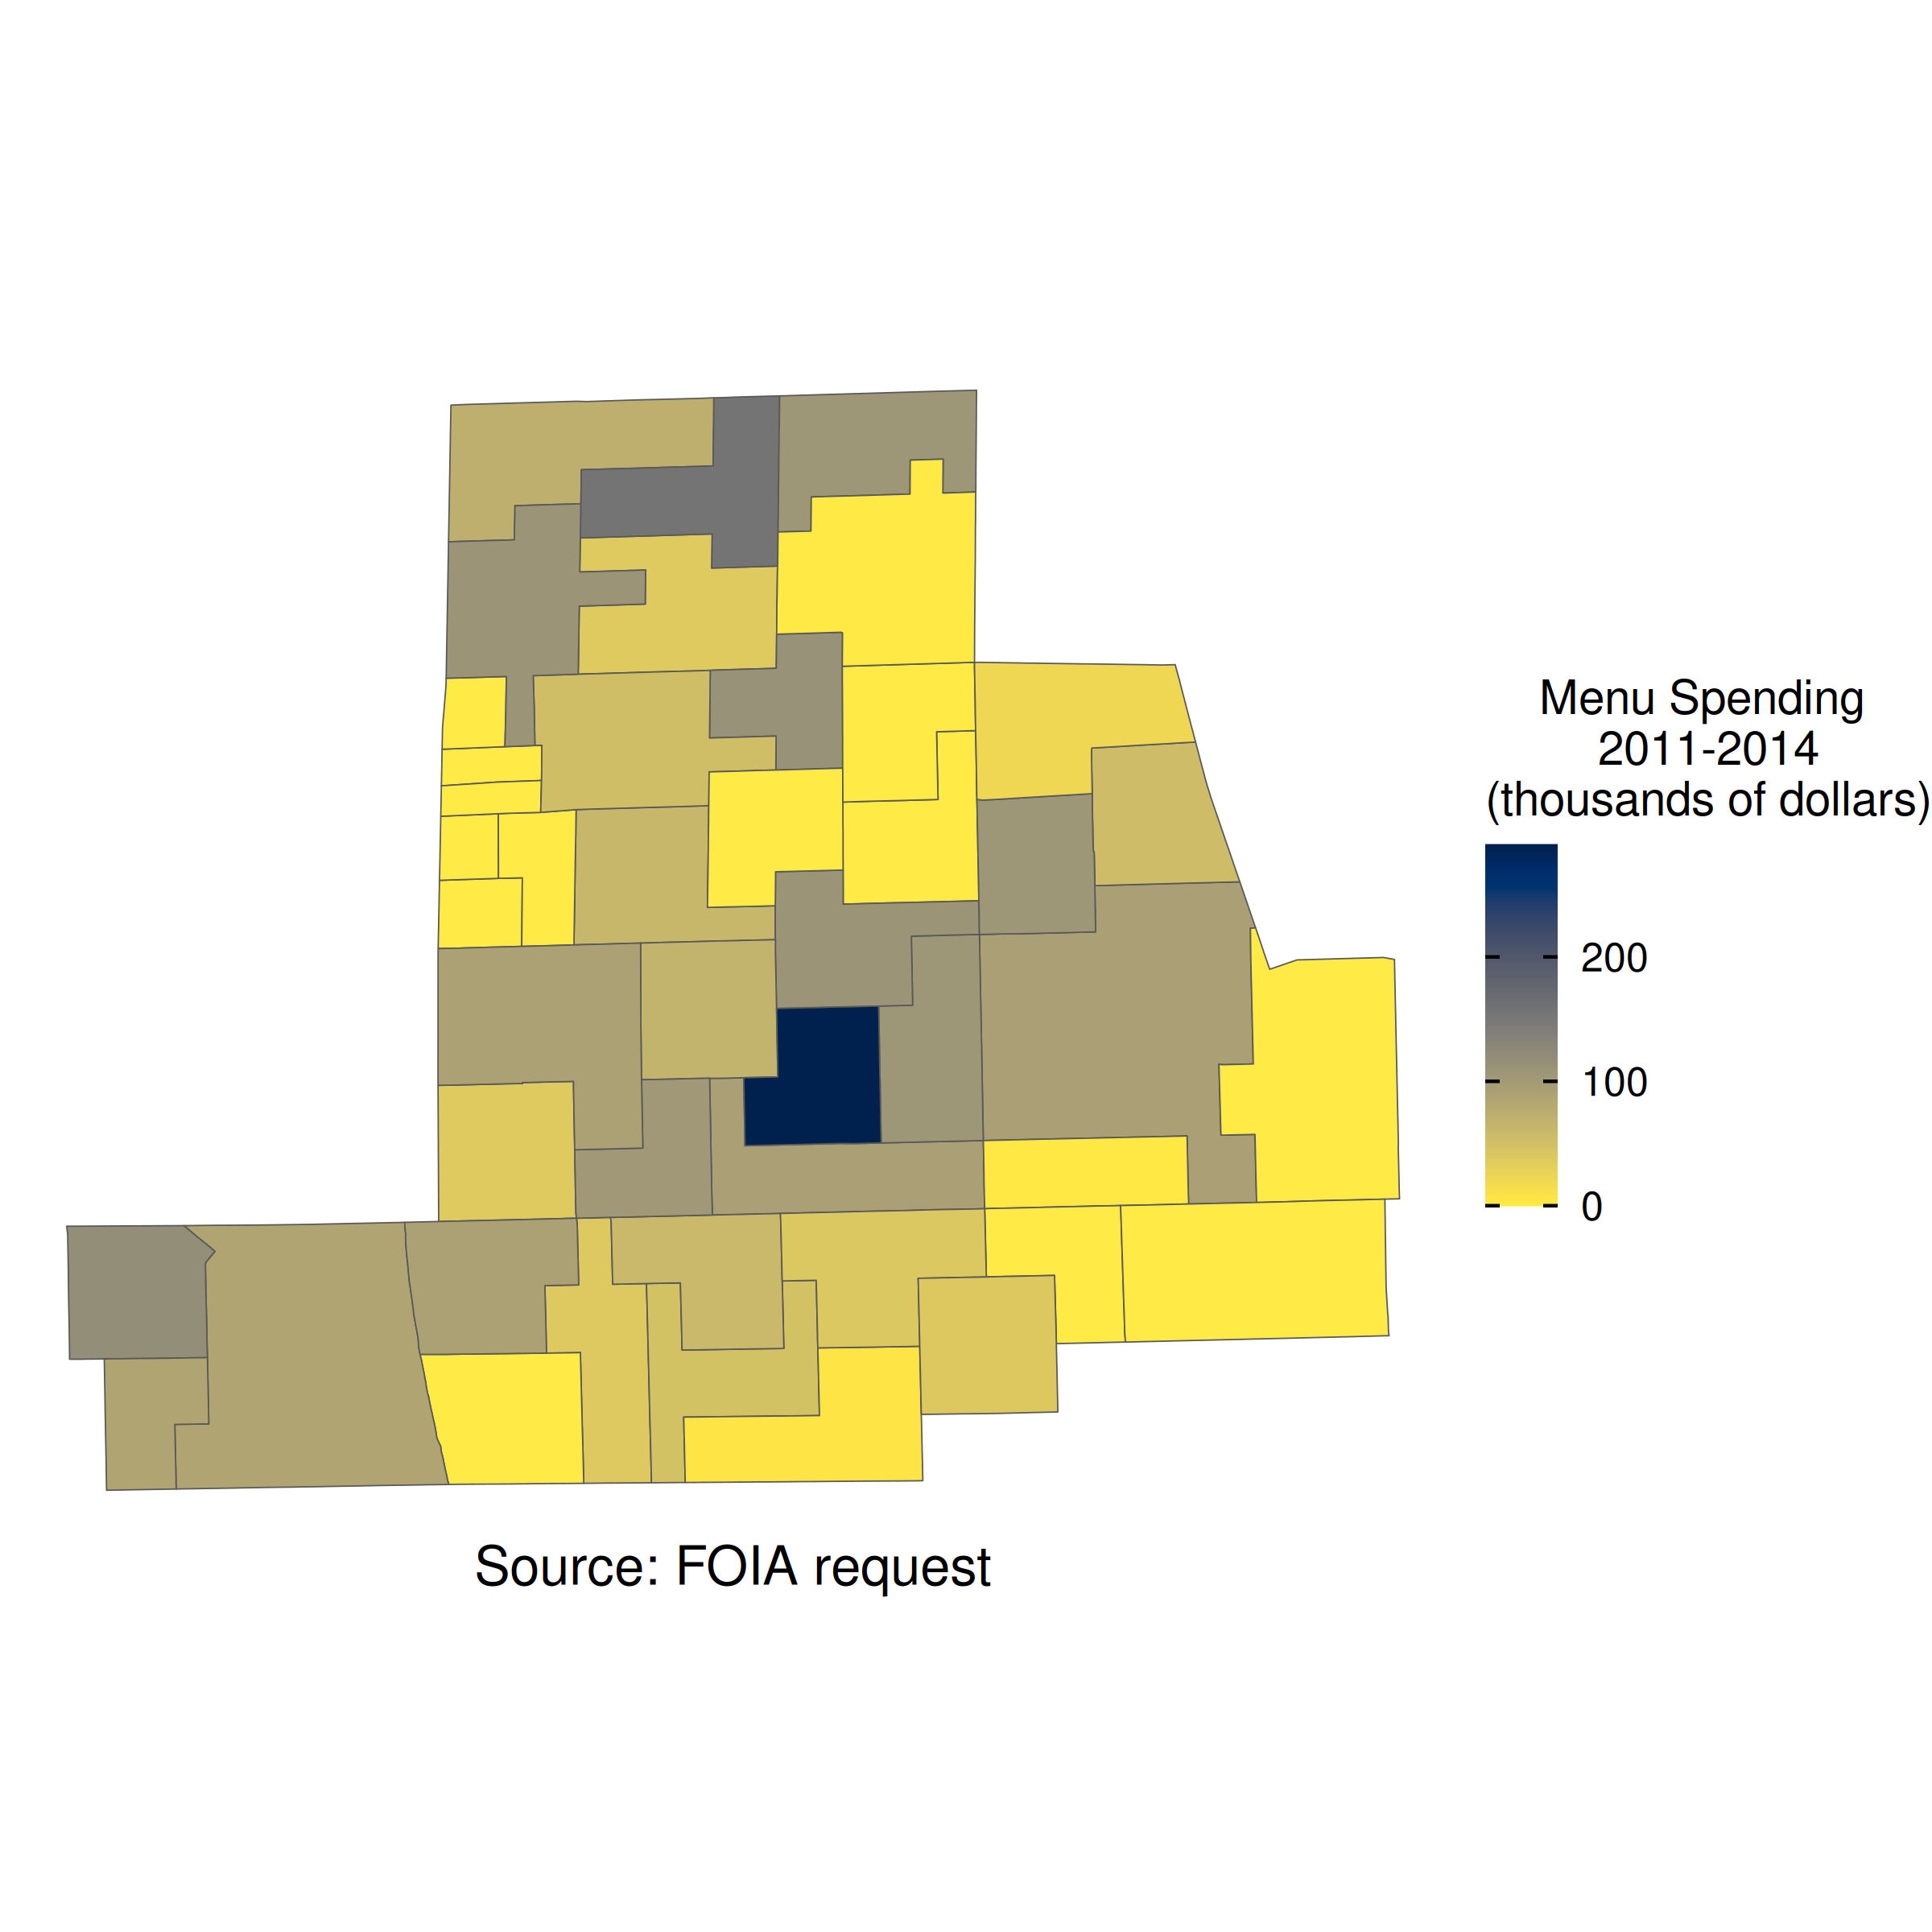
\includegraphics[width=\textwidth]{input/ward_50_menu_map_2011_2014.png}
    \caption{50th Ward Menu Allocation, 2011-2015}
    \end{subfigure}
    \caption{50th Ward Menu Allocation, 2011-2016}
    \label{fig:stone_support_maps}
\end{figure}

\textcolor{red}{\textbf{Question for Readers} Is there anything else you're curious about with this case study?}

\section*{Empirical Framework}
This section discusses the empirical framework used to analyze the data.
To determine whether aldermen are allocating spending to precincts that support them, I use a differences-in-differences approach.
However, I focus on a heterogeneous-treatment effect robust estimator.
The most standard specification is given as follows:

\begin{equation}\label{eq:standard_did}
    Y_{pt} = \alpha_{p} + \gamma_{t} + \beta T_{pt} + \epsilon{pt}
\end{equation}

Where $Y_{pt}$ is the fraction of observed spending in precinct $p$ in year $t$. $T_{pt}$ is a dummy variable that is equal to 1 if the incumbent alderman was removed by office in year $t$. $\alpha_{p}$ and $\gamma_{t}$ are precinct and year fixed effects respectively. $\epsilon_{pt}$ is the error term.
$\beta$ represents how much spending on an average precinct in the sample changes after an alderman is removed from office.
Under parallel trends, this represents the causal impact of removing an alderman from office on spending in the precincts contained in the sample.
Thus, if we focus on primarily supporting precincts, then a negative $\beta$ would indicate that the incumbent alderman was allocating more spending to the precincts that supported them than the following alderman would have chosen.
Yet, this model should not be naively applied due to the recent literature on heterogeneous treatment effects in differences-in-differences designs.
The growing literature shows that the standard two-way fixed effects estimator biases the coefficient $\beta$, is a weighted average of several differences-in-differences that compare how $Y_{pt}$ progress across pairs of groups, of which some of them can be treated in both periods \cite{chaisetwfe} \cite{CALLAWAY2021200}. 
To address this issue, I use the heterogeneous-treatment effect robust estimator proposed by \cite{CALLAWAY2021200}.

This paper estimates four variations of Equation~\ref{eq:standard_did}. 
The first two rely on a close-election assumption to justify the parallel trends assumption. 
By focusing only on wards where the incumbent alderman won by a small margin, we can assume that incumbent aldermen who win by a small margin have similar characteristics to those who lose by a small margin.
For this study, we use a margin of victory of 10\% or less to define a close election, this corresponds to approximately 300 votes in either election.
Therefore, they should behave similarly in the run-up to the election as they have similar expectations of winning.
We then examine two sets of precincts. 
The first set of precincts is the top quintile (8) precincts by vote margin in the 2015 or 2019 election for each ward whichever is appropriate to the treatment group. 
The second set of precincts is the bottom quintile precincts by vote margin in the 2015 or 2019 election for each ward, whichever is appropriate to the treatment group.
We use the 2012 through 2022 years to estimate this model, due to the 2011 redistricting complicating the use of 2005-2011 data. 

The second two variations rely on a simultaneous set of indictments of aldermen in 2019, causing three aldermen to either be ineligible for reelection, or to retire. 
We compare this group to a set of 10 control aldermen who were not indicted, have been in office for at least 10 years, and won reelection in 2019 in the general election, indicating that they were not in a competitive election. 
To measure whether or not a precinct supported an alderman, we use the total number of campaign contributions donated to the aldermen in the 2015 and 2019 elections from the precinct.
We do this because many of the ``entrenched'' aldermen have not faced a competitive election in decades, so we cannot use the vote margin to determine whether or not a precinct supported an alderman.
Despite this, all aldermen still accept campaign contributions even when there is no challenger, so we can use this as a proxy for support.
In this case, we expect that the trends for the indicted and control aldermen will be the same, as they are all not in competitive elections and thus their spending preferences should both be stable over time.
Furthermore, the unexpected nature of indictments should preclude any anticipatory behavior.
In both cases I cluster standard errors at the ward level, as that is the level at which the treatment is assigned.

\textcolor{red}{\textbf{Question for Readers} Do you have any other ideas for related questions I can explore with this data? Is there anything I'm obviously doing wrong here?}

\section*{Results and Discussion}

Starting with a simple TWFE estimate of the impact of additional off-menu expenditures, we conduct a discrete-choice analysis similar to that of \cite{berry1994}. 
Thus we conduct a simple logit model using off-menu expenditures (measured in \$ 100,00). 
This model results in the following simple regression results shown below, showing an increase in off-menu expenditures the year before an election matter and helps move the outcome towards the incumbent. 
If the results below were causal in the OLS case, this would mean that by spending the entire \$1.3M on off-menu projects, an alderperson could expect to increase their vote share from 30\% to 95\%. We further replicate the results with a direct beautification measure, which only counts public art and park spending.
 The results of substituting off-menu expenditures with beautification are shown in table 6 in the appendix. 
 Finally, the results were replicated with the 12 unopposed candidates, and the results were all statistically insignificant in that model. 
 These are shown in table 7 in the appendix.


\begin{table}[H] \centering 
  \caption{Impact of Off-Menu Expenditures with Binomial Choice, OLS, and with experience controls} 
  \label{} 
\begin{tabular}{@{\extracolsep{5pt}}lccc} 
\\[-1.8ex]\hline 
\hline \\[-1.8ex] 
 & \multicolumn{3}{c}{\textit{Model:}} \\ 
\cline{2-4} 
\\[-1.8ex] & Binomial Choice & OLS & Experience OLS\\ 
\\[-1.8ex] & (1) & (2)\\ 
\hline \\[-1.8ex] 
 off\_menu & 0.239$^{**}$ & 5.578$^{**}$ & 4.570$^{*}$ \\ 
  & (0.099) & (2.322) & (2.514) \\ 
  & & & \\ 
 exp &  &  & $-$0.377 \\ 
  &  &  & (0.363) \\ 
  & & & \\ 
 Constant & $-$0.855$^{*}$ & 30.163$^{**}$ & 35.830$^{**}$ \\ 
  & (0.497) & (11.593) & (12.799) \\ 
  & & & \\ 
\hline \\[-1.8ex] 
Observations & 71 & 71 & 71 \\ 
R$^{2}$ & 0.864 & 0.846 & 0.853 \\ 
Adjusted R$^{2}$ & 0.586 & 0.531 & 0.533 \\ 
Residual Std. Error & 0.328 (df = 23) & 7.651 (df = 23) & 7.639 (df = 22) \\ 
F Statistic & 3.107$^{***}$ (df = 47; 23) & 2.689$^{***}$ (df = 47; 23) & 2.664$^{***}$ (df = 48; 22) \\ 
\hline 
\hline \\[-1.8ex] 
\textit{Note:}  & \multicolumn{3}{r}{$^{*}$p$<$0.1; $^{**}$p$<$0.05; $^{***}$p$<$0.01} \\ 
\end{tabular} 
\end{table} 

The results of the regression discontinuity analysis are given below. 
For this we used 4 bandwidth specifications, a ``full'' bandwidth that uses the entire data-set, an Imbens-Kalyanaraman bandwidth \cite{IK_bandwidth}, a mean-square-error(MSE) optimal bandwidth derived by Calonico et al.
 \cite{CCF_MSE}, and a coverage-error-probability (CER) optimal bandwidth derived by Calonico et al \cite{CCF_CER}. 
 The results show a large and barely significant effect of an incumbent just winning the election, regardless of the bandwidth size. 
 This result indicates that when the incumbent barely wins an election, this causes off-menu expenditures to decrease by more than \$100,000 relative to wards where challengers just barely beat out incumbents if the assumptions of continuity and random assignment close to the cutoff hold. 
 These results, if they are to be trusted, perhaps show potential problems with our supposed electoral mechanism. 
 If an electoral competency mechanism drove these results, then the results should show that there is no significant difference between alderpeople who just barely won and lost the election. 
 This is because if the voters split evenly between the two candidates, then it must be the case that they have practically equivalent competence. 
 However, as we will see, these results are not as steady as the p-value may indicate. 

 
% Table created by stargazer v.5.2.3 by Marek Hlavac, Social Policy Institute. E-mail: marek.hlavac at gmail.com
% Date and time: Tue, Jan 24, 2023 - 08:33:56 PM
\begin{table}[H] \centering 
  \caption{Regression Discontinuity Results for a Variety of Bandwidths} 
  \label{rdd_cutoff_table} 
\small 
\begin{tabular}{@{\extracolsep{0pt}}lcccc} 
\\[-1.8ex]\hline 
\hline \\[-1.8ex] 
 & \multicolumn{4}{c}{Bandwidth Criterion:} \\ 
\cline{2-5} 
\\[-1.8ex] & \multicolumn{4}{c}{OffMenu} \\ 
 & Full & IK & MSE & CER \\ 
\\[-1.8ex] & (1) & (2) & (3) & (4)\\ 
\hline \\[-1.8ex] 
 IW & $-$111,845$^{**}$ & $-$129,425$^{***}$ & $-$173,271$^{***}$ & $-$152,452$^{***}$ \\ 
  & (47,501) & (38,302) & (46,566) & (49,220) \\ 
  & & & & \\ 
 IVS & 919,463$^{*}$ & 1,551,752$^{**}$ & 1,679,313$^{*}$ & 1,863,734 \\ 
  & (545,557) & (624,376) & (849,169) & (1,181,661) \\ 
  & & & & \\ 
 IW:IVS & $-$839,454 & $-$1,564,804$^{**}$ & 38,509 & $-$1,378,414 \\ 
  & (549,719) & (671,145) & (1,129,667) & (1,484,783) \\ 
  & & & & \\ 
 Constant & 140,967$^{***}$ & 159,083$^{***}$ & 161,626$^{***}$ & 164,978$^{***}$ \\ 
  & (44,467) & (33,981) & (38,497) & (40,705) \\ 
  & & & & \\ 
\hline \\[-1.8ex] 
Observations & 123 & 69 & 49 & 45 \\ 
R$^{2}$ & 0 & 0 & 0 & 0 \\ 
Adjusted R$^{2}$ & 0 & 0 & 0 & 0 \\ 
Residual Std. Error & 117,476 (df = 119) & 81,839 (df = 65) & 89,492 (df = 45) & 87,740 (df = 41) \\ 
F Statistic & 2 (df = 3; 119) & 4$^{***}$ (df = 3; 65) & 5$^{***}$ (df = 3; 45) & 4$^{**}$ (df = 3; 41) \\ 
\hline 
\hline \\[-1.8ex] 
\textit{Note:}  & \multicolumn{4}{r}{$^{*}$p$<$0.1; $^{**}$p$<$0.05; $^{***}$p$<$0.01} \\ 
\end{tabular} 
\end{table} 


The visual results of the regression discontinuity analysis are given below. 
Note how neither of the two assumptions required for the validity of the regression discontinuity design seems to hold. 
Firstly, the result is driven mainly by a large grouping of zero values to the left of the cutoff, indicating a non-random assignment. 
Secondly, there seems to be a significant increase in density right after the cutoff, indicating sorting issues. 
Finally, the data seems incredibly dispersed and can hardly be considered continuous. 

\begin{figure}[H]
    \centering
    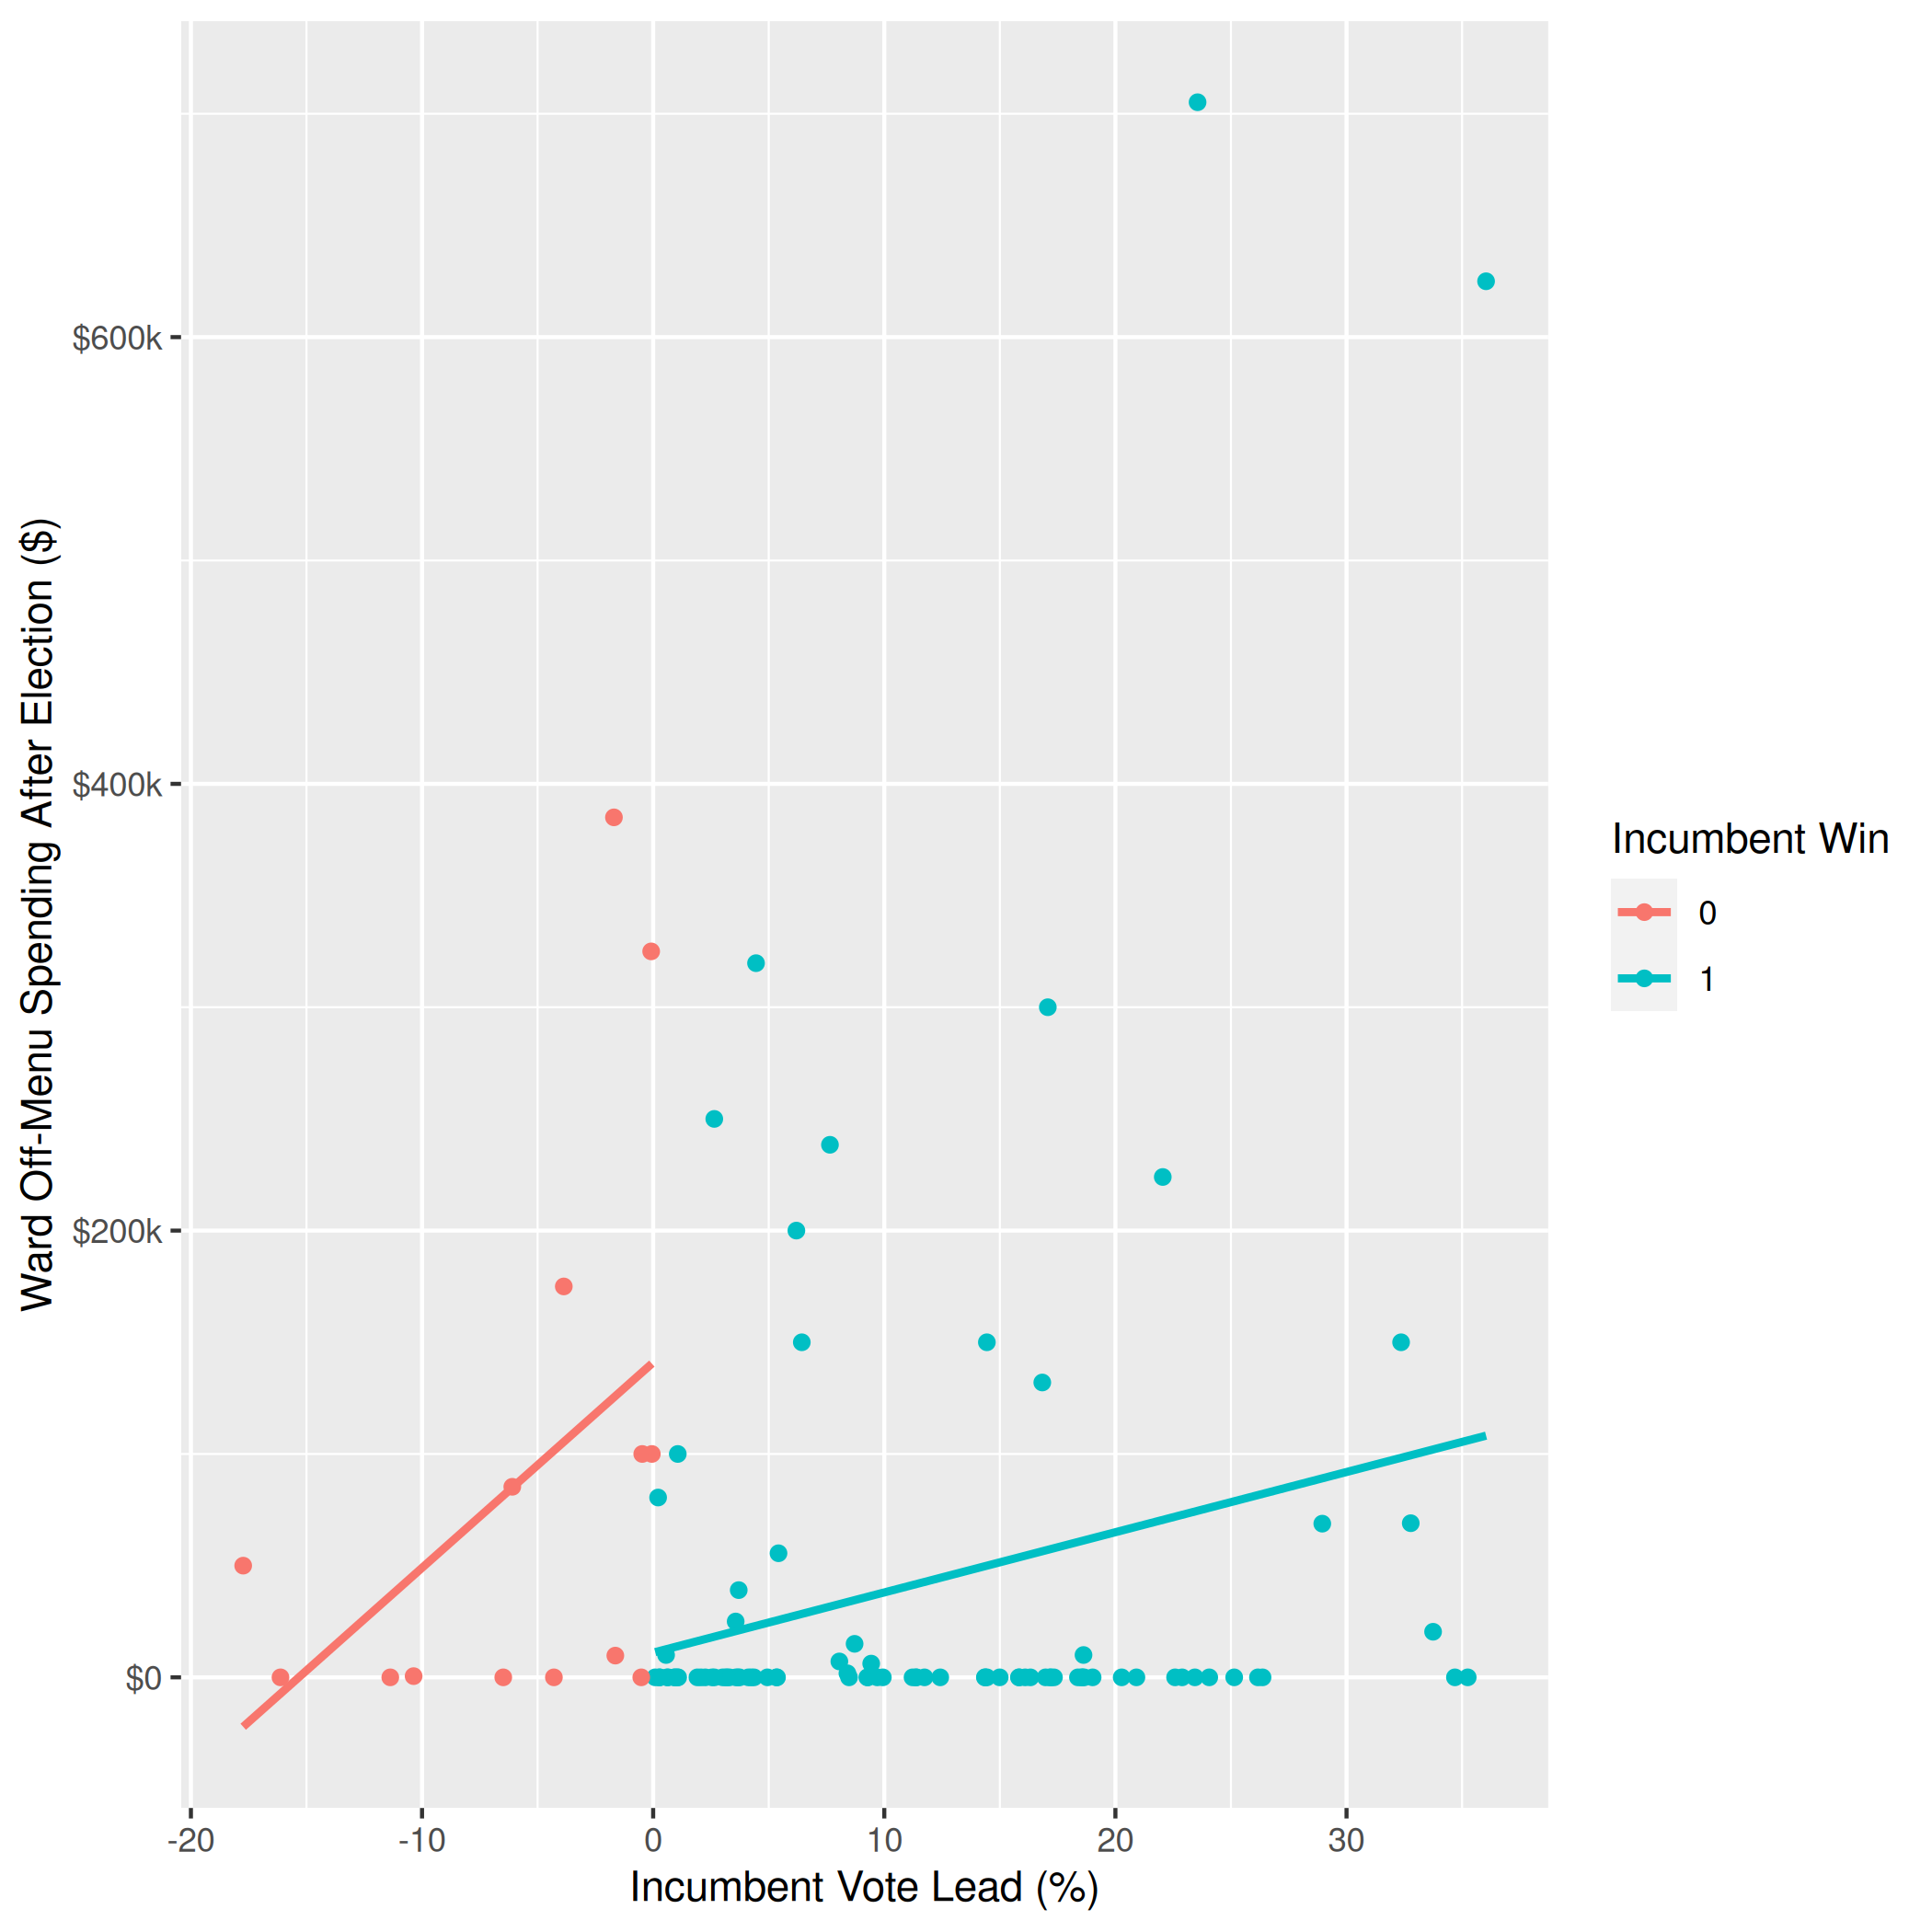
\includegraphics[scale=0.8]{input/RDD_plot.png}
        \caption{RDD results across 2011, 2015, and 2019 elections on off-menu expenditures}
\end{figure}

To verify the integrity of the regression discontinuity analysis, we perform two diagnostic procedures: A Mccrary-density test and a placebo test \cite{MCCRARY2008698}. 
The Mccrary-density test is intended to verify the random-assignment assumption, and the placebo test is intended to verify the continuity assumption. 
Starting with the Mccrary density test, we see that the visual intuition was correct. 
There is a large and statistically significant discontinuity in data density at the cutoff. 
The P-Value generated from the McCrary test is 0.00354, well below the 0.05 significance level. 
This result may be from retirement selection or the endorsement-selection reasons discussed in the methodology section. 
However, regardless of the reason for the gap, this is a significant indication that the regression discontinuity analysis is flawed.

\begin{figure}[H]
    \centering
    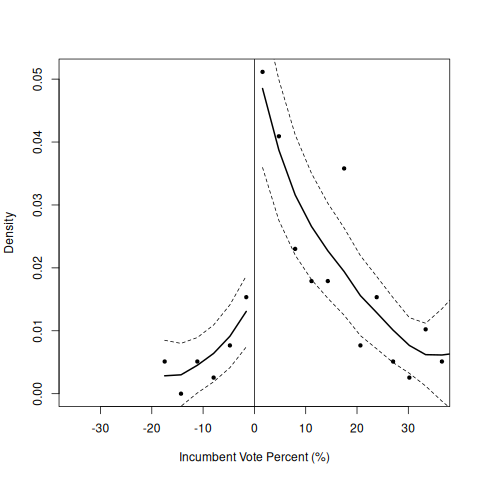
\includegraphics[scale=0.7]{input/rdd_density.png}
    \caption{Mccrary Density Test Plot}
\end{figure}

Next, we conducted a placebo test on the right side of the cutoff (due to a lack of examples of the challenger winning on the left side of the cutoff). 
We find that estimated effects range from being staunchly positive to highly negative as we move further away from the cutoff. 
However, out of 20 placebo tests, 5 achieve statistically significant levels, which is deeply concerning as it may indicate that the data generating process is inherently discontinuous, so the assumption of continuity concerning the running variable may be violated. 

\begin{figure}[H]
    \centering
    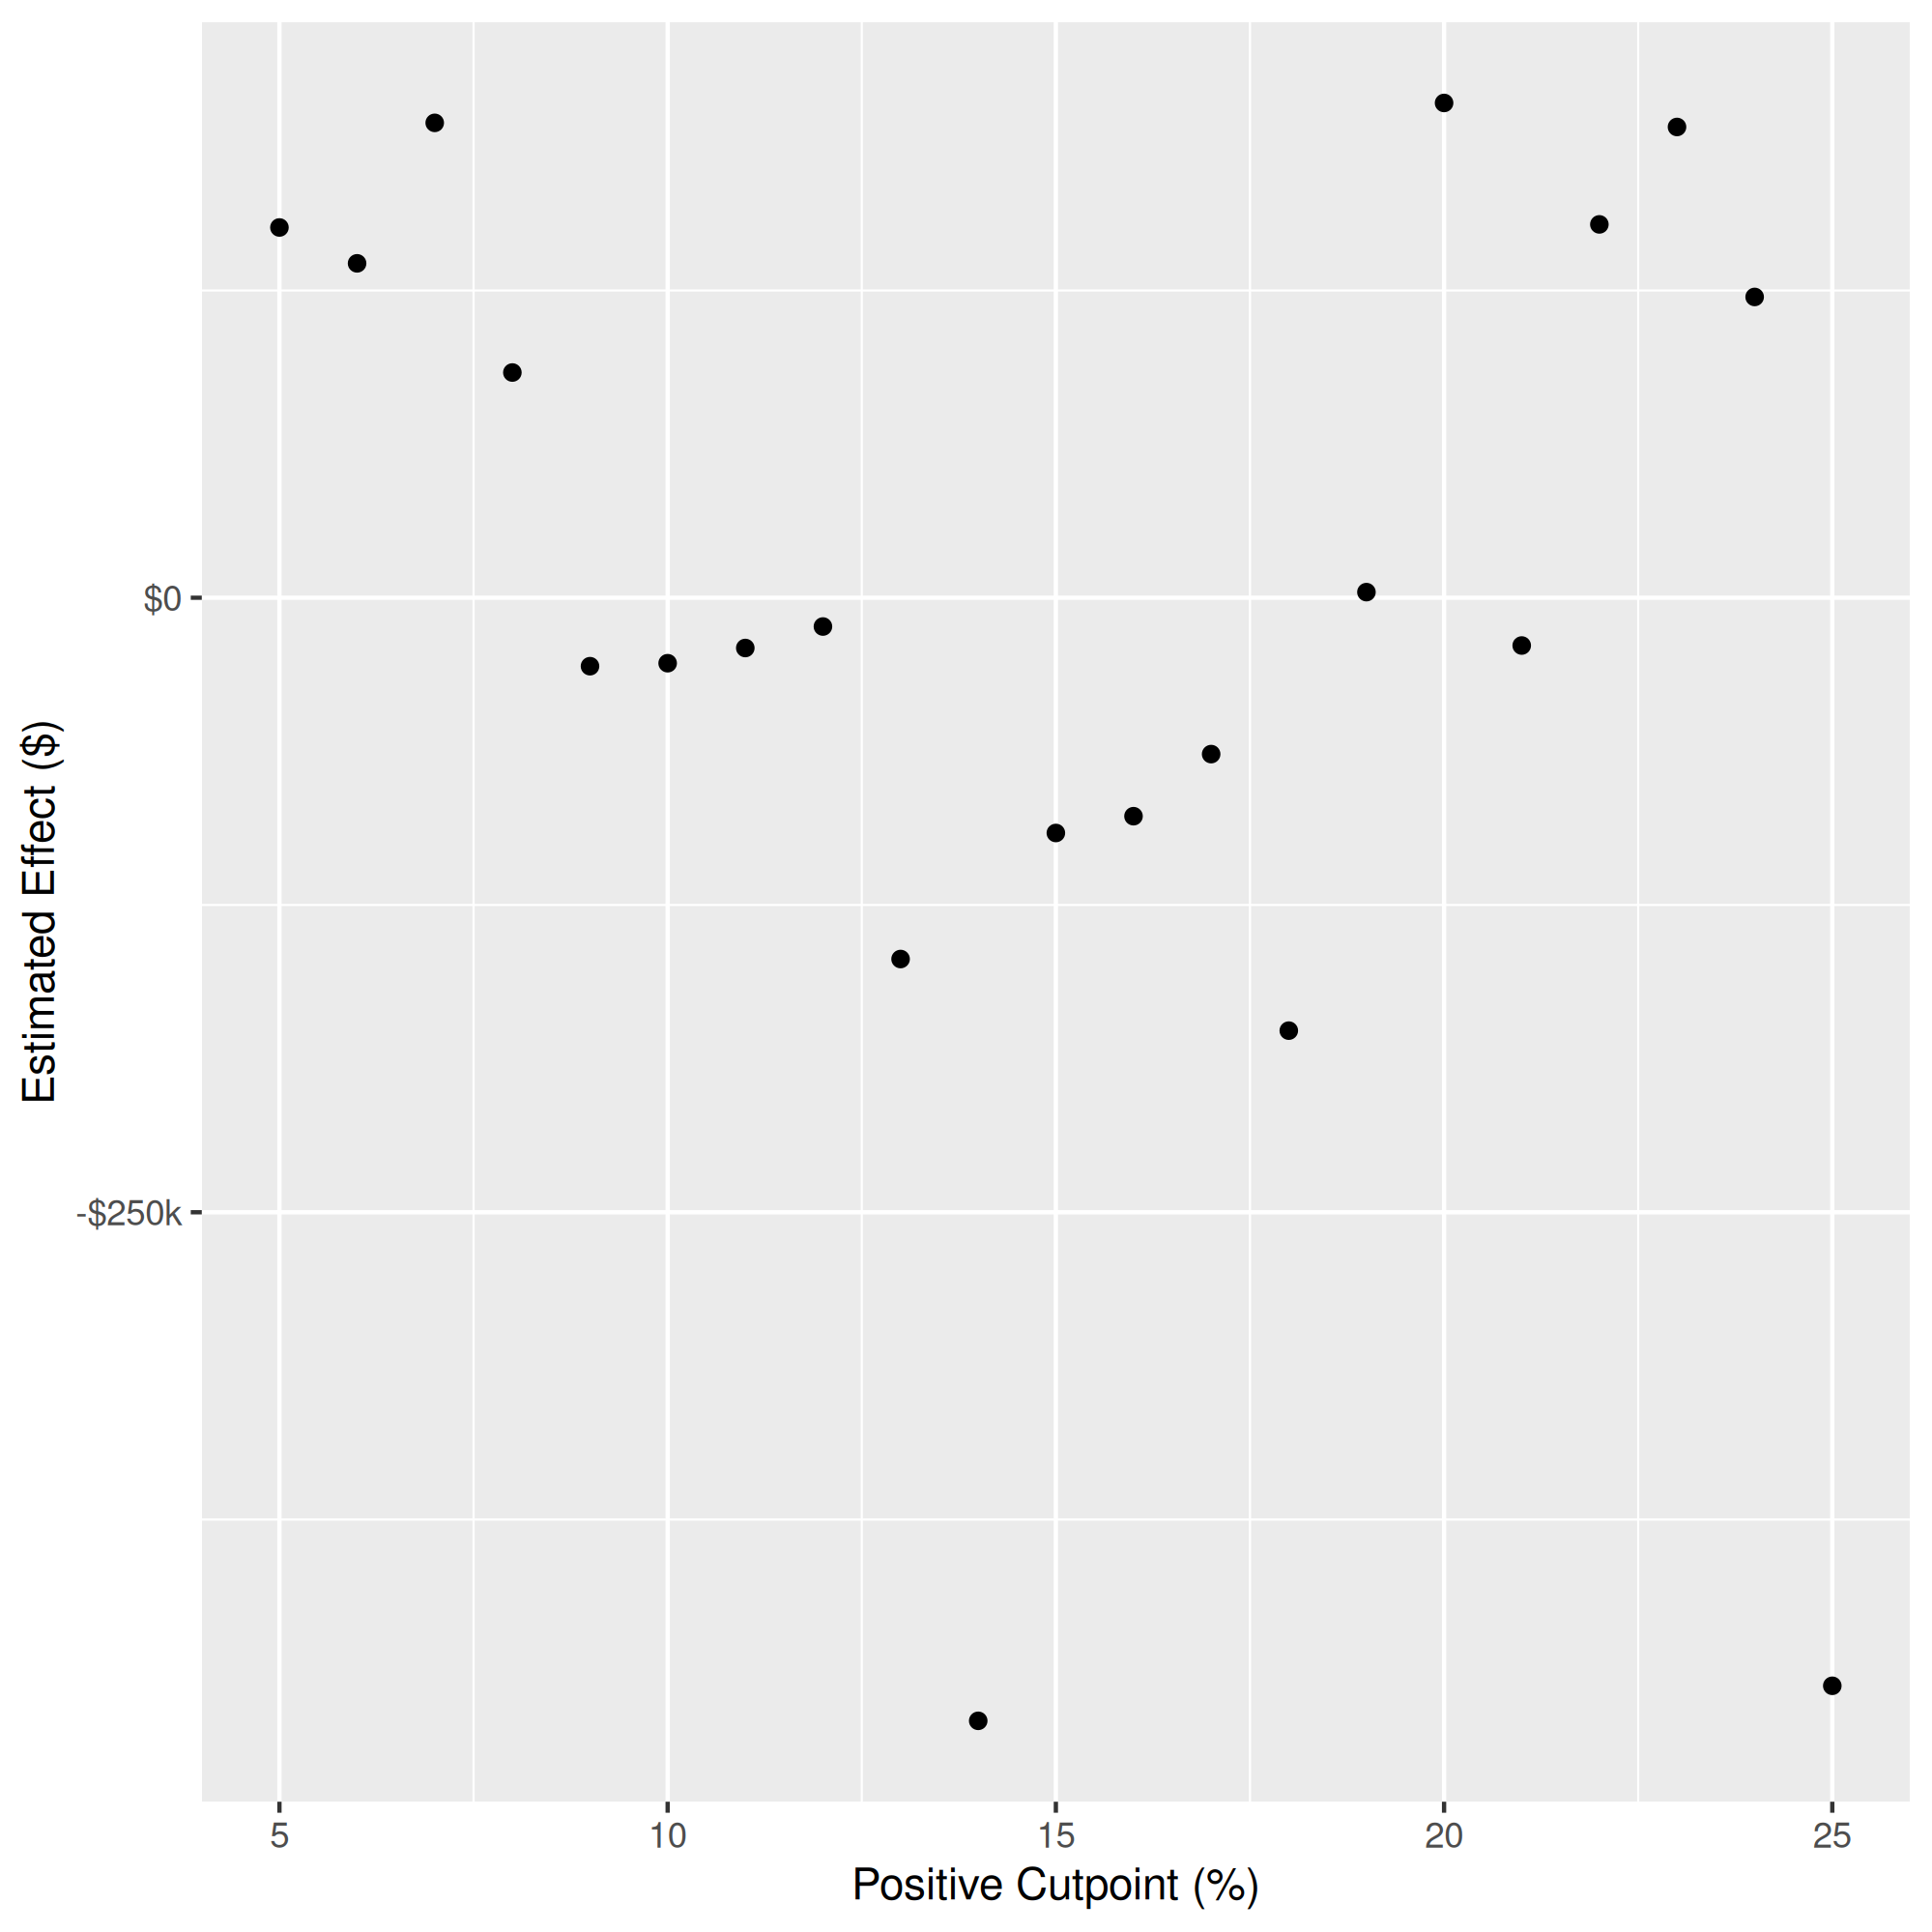
\includegraphics[scale=0.8]{input/placebo_test_effects.png}
    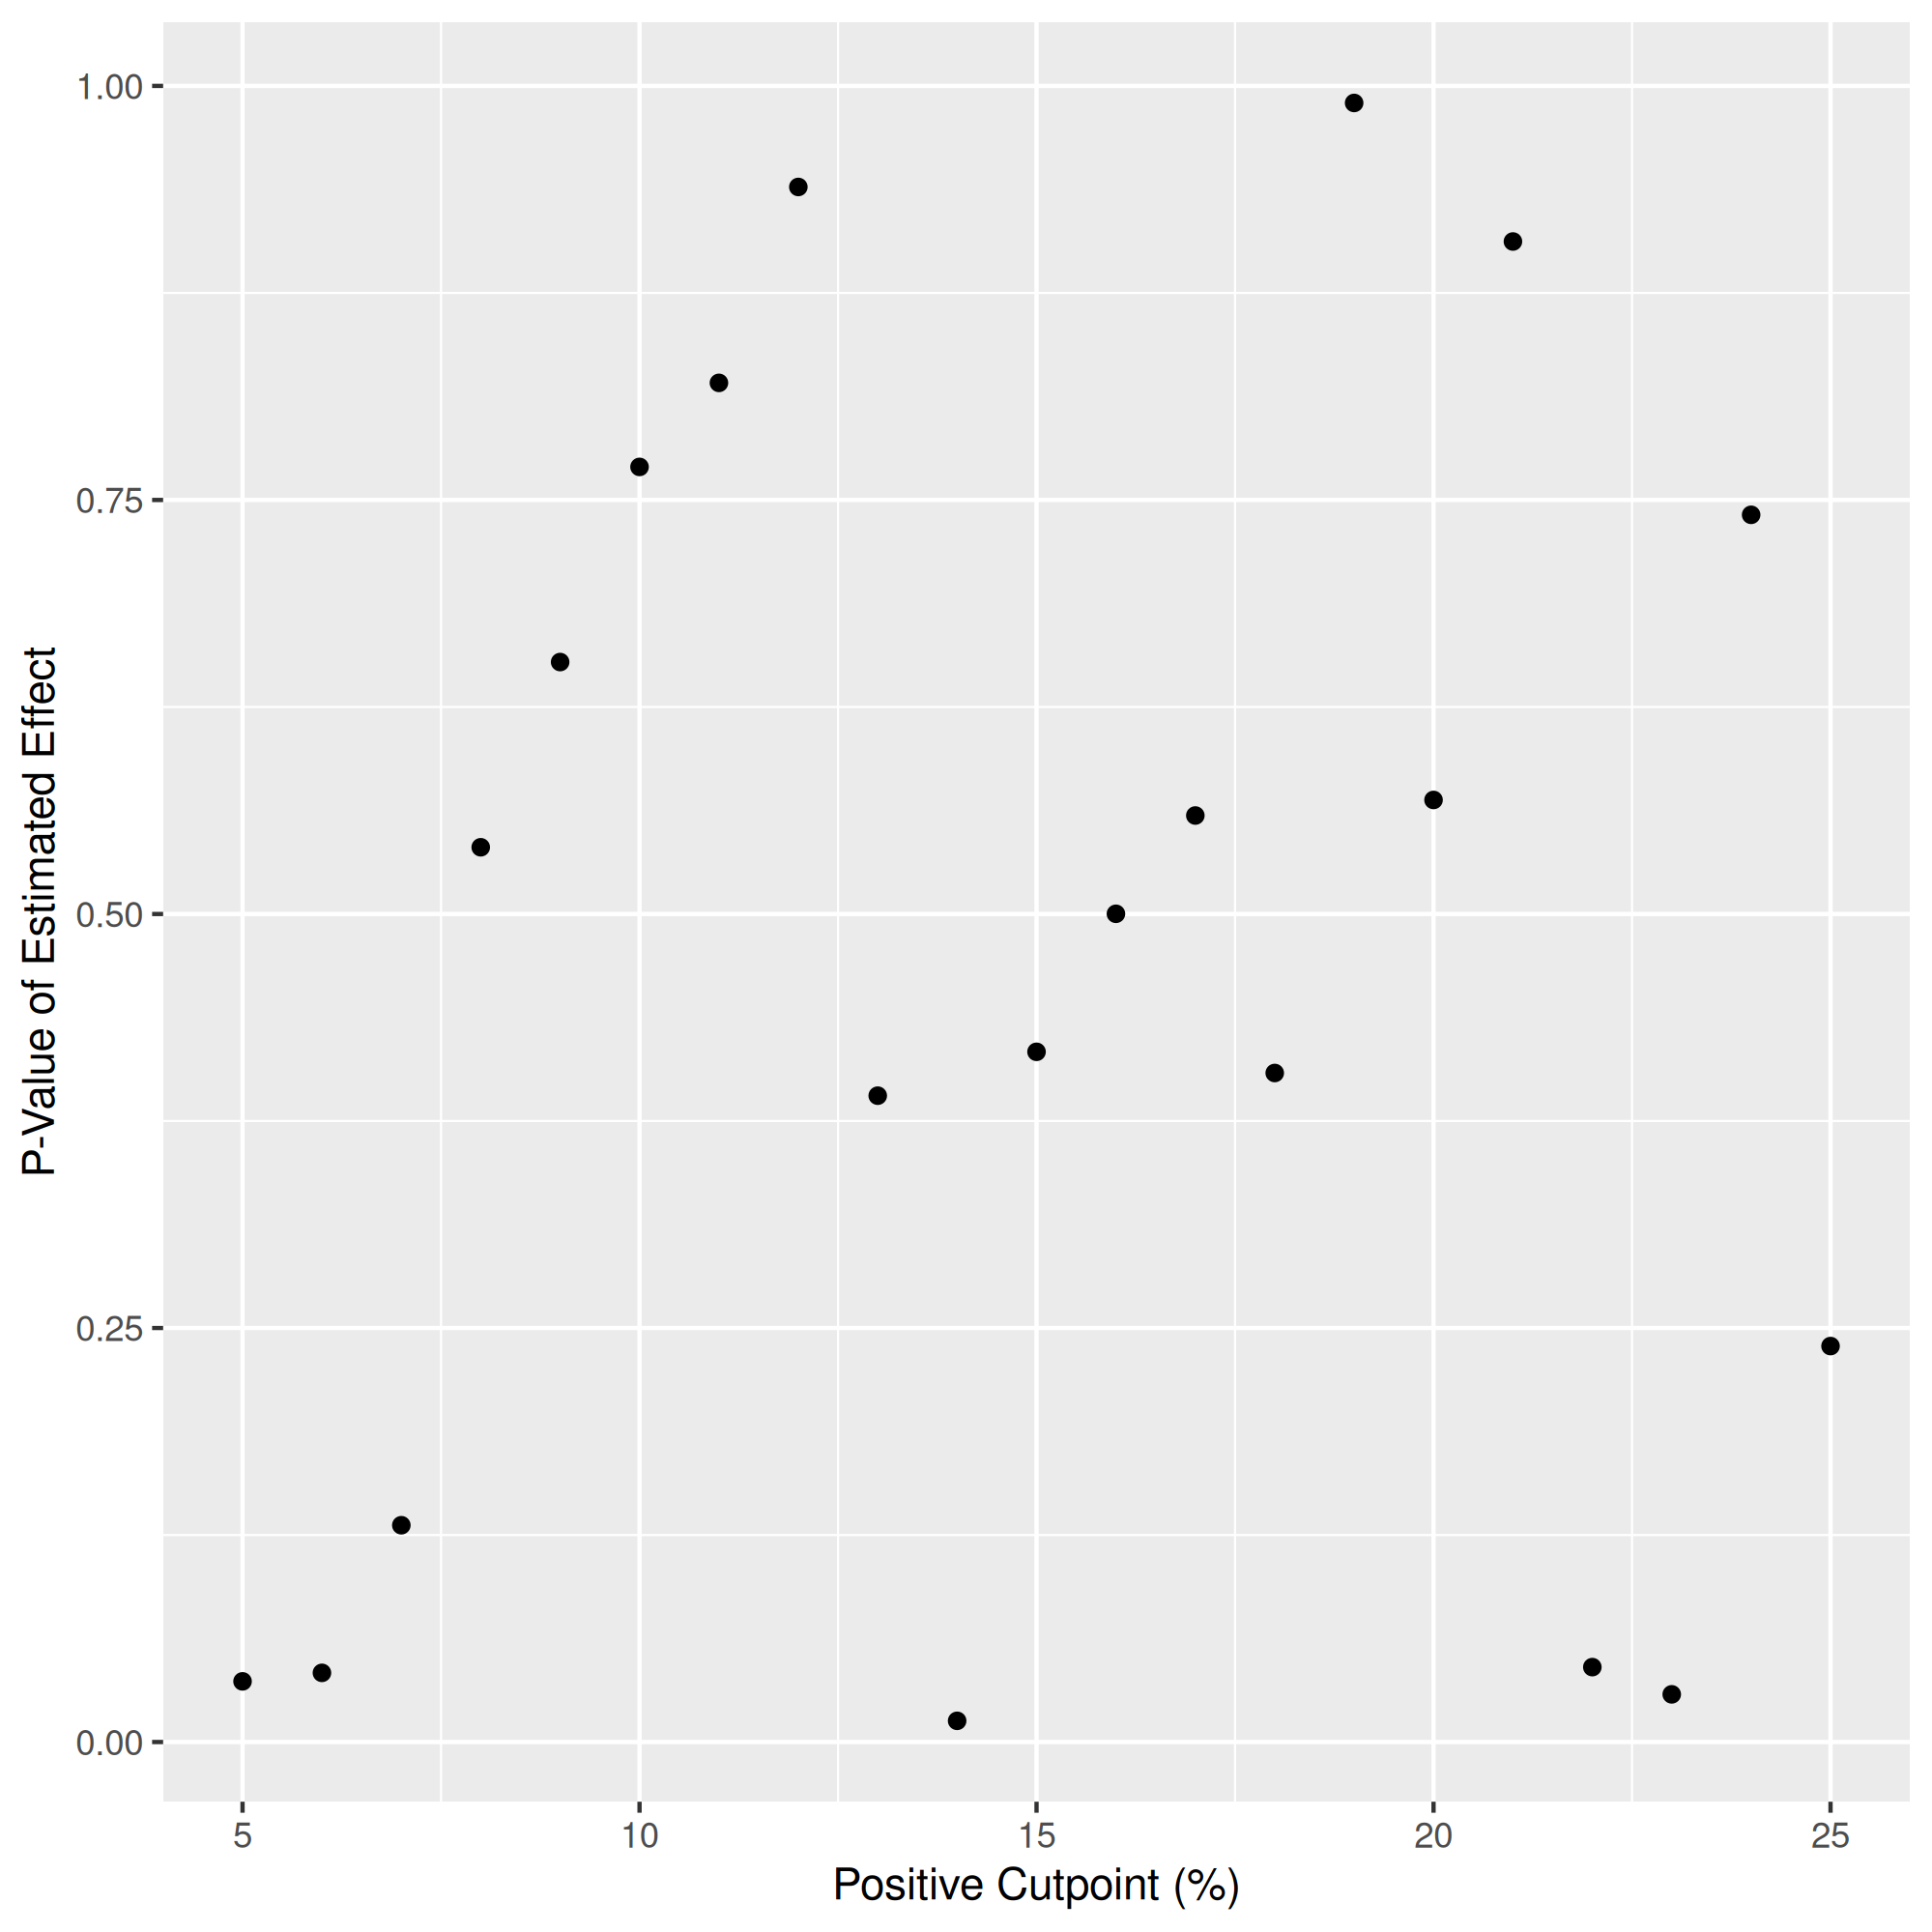
\includegraphics[scale=0.8]{input/placebo_test_pvalue.png}
    \caption{Placebo Test Results}
\end{figure}

Now moving towards diff-in-diff analysis, we show the development of the treated and non-treated wards, where treated wards are the 12 wards where the previous alderman either was elected out of the office or retired in 2015. 
From the plot, off-menu expenditures track between both groups closely prior to 2016 and then take a significant increase. 
Note that alderpersons typically take over control of the menu fund the year after they get elected \cite{particpatory_budgeting_scrapping} since they asked to approve the budget of their predecessor. 
Thus, this plot can be seen as profoundly consistent with the concept that newer alderpersons tend to spend more on off-menu expenditures. 


\begin{figure}[H]
    \centering
    \includegraphics[scale=0.8]{input/did_plot.png}
    \caption{Line plot of Off-menu expenditures}
\end{figure}

The results of the simple TWFE DiD analysis are given below in table 5. 
We include three specifications, one that uses all data and treats retiring alderpersons and council members elected out of office equally, and one reduced specification for each treatment. 
$treated_1$ is the dummy variable indicating that a group is in the post-period of 2016 on-wards and is in the treatment group. 
Each subsequent $treated$ variable estimates the effect in the post-period, so $treated_2$ is the estimate for the 2017 period, and so on. 
The 50 data points from 2020 are excluded due to the 2019 election. 

% Table created by stargazer v.5.2.3 by Marek Hlavac, Social Policy Institute. E-mail: marek.hlavac at gmail.com
% Date and time: Tue, Jun 21, 2022 - 04:53:19 PM
\begin{table}[H] \centering 
  \caption{TWFE DiD specification} 
  \label{} 
\begin{tabular}{@{\extracolsep{5pt}}lccc} 
\\[-1.8ex]\hline 
\hline \\[-1.8ex] 
 & \multicolumn{3}{c}{\textit{Dependent variable:}} \\ 
\cline{2-4} 
\\[-1.8ex] & \multicolumn{3}{c}{off menu expenditures} \\ 
\\[-1.8ex] & Both & Elected Only & Retired Only\\ 
\hline \\[-1.8ex] 
 treated\_1 & 116,597.900$^{***}$ & 98,598.880$^{**}$ & 87,257.720 \\ 
  & (37,476.320) & (48,054.550) & (54,096.760) \\ 
  & & & \\ 
 treated\_2 & 76,880.010$^{**}$ & 27,719.370 & 41,346.880 \\ 
  & (37,476.320) & (48,054.550) & (54,096.760) \\ 
  & & & \\ 
 treated\_3 & 46,261.560 & 11,758.780 & 39,047.440 \\ 
  & (37,476.320) & (48,054.550) & (54,096.760) \\ 
  & & & \\ 
 treated\_4 & 22,180.280 & $-$60,015.080 & 47,998.510 \\ 
  & (37,476.320) & (48,054.550) & (54,096.760) \\ 
  & & & \\ 
 Constant & 401,848.100$^{***}$ & 51,387.300$^{**}$ & 401,106.800$^{***}$ \\ 
  & (38,318.320) & (22,857.340) & (38,839.330) \\ 
  & & & \\ 
\hline \\[-1.8ex] 
Observations & 400 & 360 & 328 \\ 
R$^{2}$ & 0.432 & 0.029 & 0.455 \\ 
Adjusted R$^{2}$ & 0.331 & $-$0.005 & 0.354 \\ 
Residual Std. Error & 101,227.700 (df = 339) & 128,918.500 (df = 347) & 101,381.900 (df = 276) \\ 
F Statistic & 4.296$^{***}$ (df = 60; 339) & 0.849 (df = 12; 347) & 4.511$^{***}$ (df = 51; 276) \\ 
\hline 
\hline \\[-1.8ex] 
\textit{Note:}  & \multicolumn{3}{r}{$^{*}$p$<$0.1; $^{**}$p$<$0.05; $^{***}$p$<$0.01} \\ 
\end{tabular} 
\end{table} 
The ATT(g,t) analysis results are depicted below, only for the full specification, including both treatments as equal. 
When the incumbent lost control of the fund in 2016, we observed a large increase in off-menu expenditures that is barely statistically significant at a level just above \$100,000, which is similar to the results shown in the discontinuity analysis and the simple TWFE analysis above. 
Furthermore, we tested parallel pre-trends using the event study framework discussed in \cite{CALLAWAY2021200} and found that we could not reject the null hypothesis of parallel pre-trends with a p-value of 0.7754. 

\begin{figure}[H]
    \centering
    \includegraphics[scale=0.8]{input/did_treatmenteffect_plot.png}
    \caption{Treatment effect plot}
\end{figure}


However, the figure above shows that the spike is largest after the election, and then the effect dies off before the next election. This effect is not what one would expect if the DiD estimator captured an electoral effect. 
If this were an electoral effect, we would most likely see the increase in off-menu expenditures happening right before the next election in 2018. However, that is not what we see. 
Thus, this is more likely some voter-selection effect. 
We looked into the 12 candidates who made up our treatment group and the primary issues in their campaigns. 
I found articles where four candidates cited public participation and presence as key themes of their campaign \, cite{wttw. 2015} \cite{dna.2015_18} \cite{dna.2015_35} \cite{dna.2015_7}. 
Thus, from this informal evidence and the data presented, the effect is more likely from the selection or the informational mechanisms and is unlikely to be the electoral mechanism. 
\section*{Conclusions}

Overall we find some evidence that aldermen may sometimes disproportionately allocate spending to their most supporting precincts, particularly when they are long-entrenched and not facing a competitive election.
The paper starts by verifying a rumor that a particular alderman disproportionately allocated spending to his most supporting precincts.
Then it uses two applications of a differences-in-differences research design to arrive at this fact.
The first application focuses on aldermen who lost by a small margin, and finds that the evidence for disproportionate spending is very weak.
While the magnitude of the estimated effect on the top precincts in the close election design is large, it is not even close to statistically significant, and even the sign of the effect is not robust to changes in the number of supporting/opposing precincts included in the sample.
We find that the effect is economically large and statistically significant when we use the indictment design.
The statistical significance is sensitive to parameters such as the number of supporting or opposing precincts included per ward, but the economic significance is not and stays largely the same for this design so long as you decrease the number of precincts.
This is likely due to the fact that increasing the number of precincts dilutes the average treatment effect, so it decreases the aggregated treatment effect.

The results help build on the burgeoning urban economics of infrastructure literature by showing that political incentives can distort the allocation of infrastructure spending.
Secondly, the differences between the competitive election and indictment designs show that the electoral competition can be a powerful force in constraining the clientelistic tendencies of politicians.
There is also a lesson in urban planners that while discretion can be useful, it can also be abused and lead to unintended consequences.
Therefore, the capacity for discretion should be carefully considered when designing a program.


% -----------------------------------------------
% 	REFERENCES
% -----------------------------------------------

\bibliography{../bib/bib.bib}{}

\newpage
\clearpage

\begin{center} \Large \textbf{Appendix -- For Online Publication} \end{center}
\appendix
\numberwithin{equation}{section}
\numberwithin{figure}{section}
\numberwithin{table}{section}

\section*{Appendix: Regression Results with Beautification}

\begin{table}[H] \centering 
  \caption{Discrete Choice and TWFE results with Beautification} 
  \label{} 
\begin{tabular}{lccc} 
\\[-1.8ex]\hline 
\hline \\[-1.8ex] 
 & \multicolumn{3}{c}{\textit{Model:}} \\ 
\cline{2-4} 
\\[-1.8ex] & Discrete Choice & OLS & Experience OLS \\ 
\\[-1.8ex] & (1) & (2) & (3)\\ 
\hline \\[-1.8ex] 
 beauty & 0.281$^{**}$ & 6.690$^{**}$ & 5.696$^{*}$ \\ 
  & (0.119) & (2.770) & (2.833) \\ 
  & & & \\ 
 exp &  &  & $-$0.447 \\ 
  &  &  & (0.343) \\ 
  & & & \\ 
 Constant & $-$0.941$^{*}$ & 27.667$^{**}$ & 33.379$^{**}$ \\ 
  & (0.532) & (12.345) & (12.928) \\ 
  & & & \\ 
\hline \\[-1.8ex] 
Observations & 71 & 71 & 71 \\ 
R$^{2}$ & 0.863 & 0.846 & 0.857 \\ 
Adjusted R$^{2}$ & 0.583 & 0.532 & 0.546 \\ 
Residual Std. Error & 0.329 (df = 23) & 7.643 (df = 23) & 7.530 (df = 22) \\ 
F Statistic & 3.078$^{***}$ (df = 47; 23) & 2.696$^{***}$ (df = 47; 23) & 2.755$^{***}$ (df = 48; 22) \\ 
\hline 
\hline \\[-1.8ex] 
\textit{Note:}  & \multicolumn{3}{r}{$^{*}$p$<$0.1; $^{**}$p$<$0.05; $^{***}$p$<$0.01} \\ 
\end{tabular} 
\end{table} 


\begin{table}[H] \centering 
  \caption{OLS Results with Unopposed Candidates Included} 
  \label{} 
\begin{tabular}{@{\extracolsep{5pt}}lcc} 
\\[-1.8ex]\hline 
\hline \\[-1.8ex] 
 & \multicolumn{2}{c}{\textit{Dependent variable:}} \\ 
\cline{2-3} 
\\[-1.8ex] & \multicolumn{2}{c}{Vote Share} \\ 
\\[-1.8ex] & (1) & (2)\\ 
\hline \\[-1.8ex] 
 off\_menu & 4.918 &  \\ 
  & (3.654) &  \\ 
  & & \\ 
 exp &  & $-$0.949 \\ 
  &  & (0.626) \\ 
  & & \\ 
 Constant & 32.639 & 55.827$^{***}$ \\ 
  & (20.171) & (15.028) \\ 
  & & \\ 
\hline \\[-1.8ex] 
Observations & 83 & 83 \\ 
R$^{2}$ & 0.727 & 0.731 \\ 
Adjusted R$^{2}$ & 0.301 & 0.311 \\ 
Residual Std. Error (df = 32) & 14.804 & 14.699 \\ 
F Statistic (df = 50; 32) & 1.705$^{*}$ & 1.739$^{**}$ \\ 
\hline 
\hline \\[-1.8ex] 
\textit{Note:}  & \multicolumn{2}{r}{$^{*}$p$<$0.1; $^{**}$p$<$0.05; $^{***}$p$<$0.01} \\ 
\end{tabular} 
\end{table} 



% Table created by stargazer v.5.2.3 by Marek Hlavac, Social Policy Institute. E-mail: marek.hlavac at gmail.com
% Date and time: Tue, Jan 24, 2023 - 08:33:57 PM
\begin{table}[H] \centering 
  \caption{Regression Discontinuity Results with Beautification} 
  \label{rdd_cutoff_table_beauty} 
\small 
\begin{tabular}{@{\extracolsep{0pt}}lcccc} 
\\[-1.8ex]\hline 
\hline \\[-1.8ex] 
 & \multicolumn{4}{c}{Bandwidth Criterion:} \\ 
\cline{2-5} 
\\[-1.8ex] & \multicolumn{4}{c}{beauty} \\ 
 & Full & IK & MSE & CER \\ 
\\[-1.8ex] & (1) & (2) & (3) & (4)\\ 
\hline \\[-1.8ex] 
 IW & 397 & 251 & 253 & 524 \\ 
  & (6,577) & (6,874) & (8,428) & (9,127) \\ 
  & & & & \\ 
 IVS & $-$2,016 & $-$2,016 & $-$7,480 & $-$37,940 \\ 
  & (75,033) & (75,044) & (237,448) & (342,903) \\ 
  & & & & \\ 
 IW:IVS & 1,930 & 3,542 & 11,355 & 44,949 \\ 
  & (75,725) & (79,608) & (243,401) & (354,017) \\ 
  & & & & \\ 
 Constant & 49,575$^{***}$ & 49,575$^{***}$ & 49,450$^{***}$ & 49,090$^{***}$ \\ 
  & (6,077) & (6,078) & (7,567) & (8,113) \\ 
  & & & & \\ 
\hline \\[-1.8ex] 
Observations & 4,150 & 3,250 & 2,300 & 1,900 \\ 
R$^{2}$ & 0 & 0 & 0 & 0 \\ 
Adjusted R$^{2}$ & $-$0 & $-$0 & $-$0 & $-$0 \\ 
Residual Std. Error & 103,521 (df = 4146) & 103,536 (df = 3246) & 103,532 (df = 2296) & 103,546 (df = 1896) \\ 
F Statistic & 0 (df = 3; 4146) & 0 (df = 3; 3246) & 0 (df = 3; 2296) & 0 (df = 3; 1896) \\ 
\hline 
\hline \\[-1.8ex] 
\textit{Note:}  & \multicolumn{4}{r}{$^{*}$p$<$0.1; $^{**}$p$<$0.05; $^{***}$p$<$0.01} \\ 
\end{tabular} 
\end{table} 


% Table created by stargazer v.5.2.3 by Marek Hlavac, Social Policy Institute. E-mail: marek.hlavac at gmail.com
% Date and time: Sun, Jul 17, 2022 - 03:52:33 PM
\begin{table}[H] \centering 
  \caption{Diff-in-Diff Results with Beautification} 
  \label{} 
\begin{tabular}{@{\extracolsep{5pt}}lccc} 
\\[-1.8ex]\hline 
\hline \\[-1.8ex] 
 & \multicolumn{3}{c}{\textit{Treatment Variable:}} \\ 
\cline{2-4} 
\\
\\[-1.8ex] & Both & Electoral Only & Retirement Only\\ 
\hline \\[-1.8ex] 
 treated & 96,202.610$^{***}$ & 105,220.300$^{**}$ & 81,802.030$^{*}$ \\ 
  & (33,413.550) & (41,793.240) & (47,734.510) \\ 
  & & & \\ 
 treated\_1 & $-$50,774.430 & $-$99,109.770$^{*}$ & $-$44,385.510 \\ 
  & (42,265.170) & (59,103.990) & (60,379.910) \\ 
  & & & \\ 
 treated\_2 & 8,470.087 & 33,825.860 & 17,229.070 \\ 
  & (42,265.170) & (59,103.990) & (60,379.910) \\ 
  & & & \\ 
 treated\_3 & $-$30,194.430 & $-$82,640.400 & 1,600.154 \\ 
  & (42,265.170) & (59,103.990) & (60,379.910) \\ 
  & & & \\ 
 treated\_4 & 27,918.280 & 27,503.180 & 36,145.330 \\ 
  & (42,265.170) & (59,103.990) & (60,379.910) \\ 
  & & & \\ 
 Constant & 297,785.700$^{***}$ & 56,001.950$^{***}$ & 298,376.600$^{***}$ \\ 
  & (32,512.140) & (18,688.580) & (32,644.510) \\ 
  & & & \\ 
\hline \\[-1.8ex] 
Observations & 450 & 405 & 378 \\ 
R$^{2}$ & 0.355 & 0.050 & 0.382 \\ 
Adjusted R$^{2}$ & 0.252 & 0.016 & 0.279 \\ 
Residual Std. Error & 90,253.700 (df = 387) & 107,186.800 (df = 390) & 89,606.330 (df = 323) \\ 
F Statistic & 3.440$^{***}$ (df = 62; 387) & 1.466 (df = 14; 390) & 3.696$^{***}$ (df = 54; 323) \\ 
\hline 
\hline \\[-1.8ex] 
\textit{Note:}  & \multicolumn{3}{r}{$^{*}$p$<$0.1; $^{**}$p$<$0.05; $^{***}$p$<$0.01} \\ 
\end{tabular} 
\end{table} 
%\input{./sections/appendix_data.tex}
%\input{./sections/appendix_empirics.tex}

\end{document}